\chapter{Multi-objective problems}
In real-world environments, considering a single reachability or shortest path problem might not be sufficient for some situations.
Indeed, building an optimal strategy satisfying one problem could negatively affect the results of applying this same strategy to satisfy other relevant problems.
For instance, we should be interested in a strategy that does not fail to reach a target with a cost bounded and that however optimises the expected cost to this target.
Moreover, we should also be interested in getting a strategy satisfying at a time many reachability problems, and furthermore, many percentile problems.
This chapter introduces \textit{multi-objective} problems, where we are interested in solving \textit{simultaneously} multiple sub-problems introduced in previous chapters.
\begin{example}[\textit{Communication between nodes in a wireless sensor network}]\label{main-example}
Consider a wireless sensor network containing three nodes $n_0,\, n_1$ and $n_2$. Assume that $n_0, \, n_1$ and $n_3$ are separated by the same distance, that the sensor $n_0$ has to send messages to $n_2$ at regular intervals and that a wall stands between $n_0$ and $n_2$ (cf. Figure \ref{sensor_net}).
\begin{figure}[h!]
  \centering
  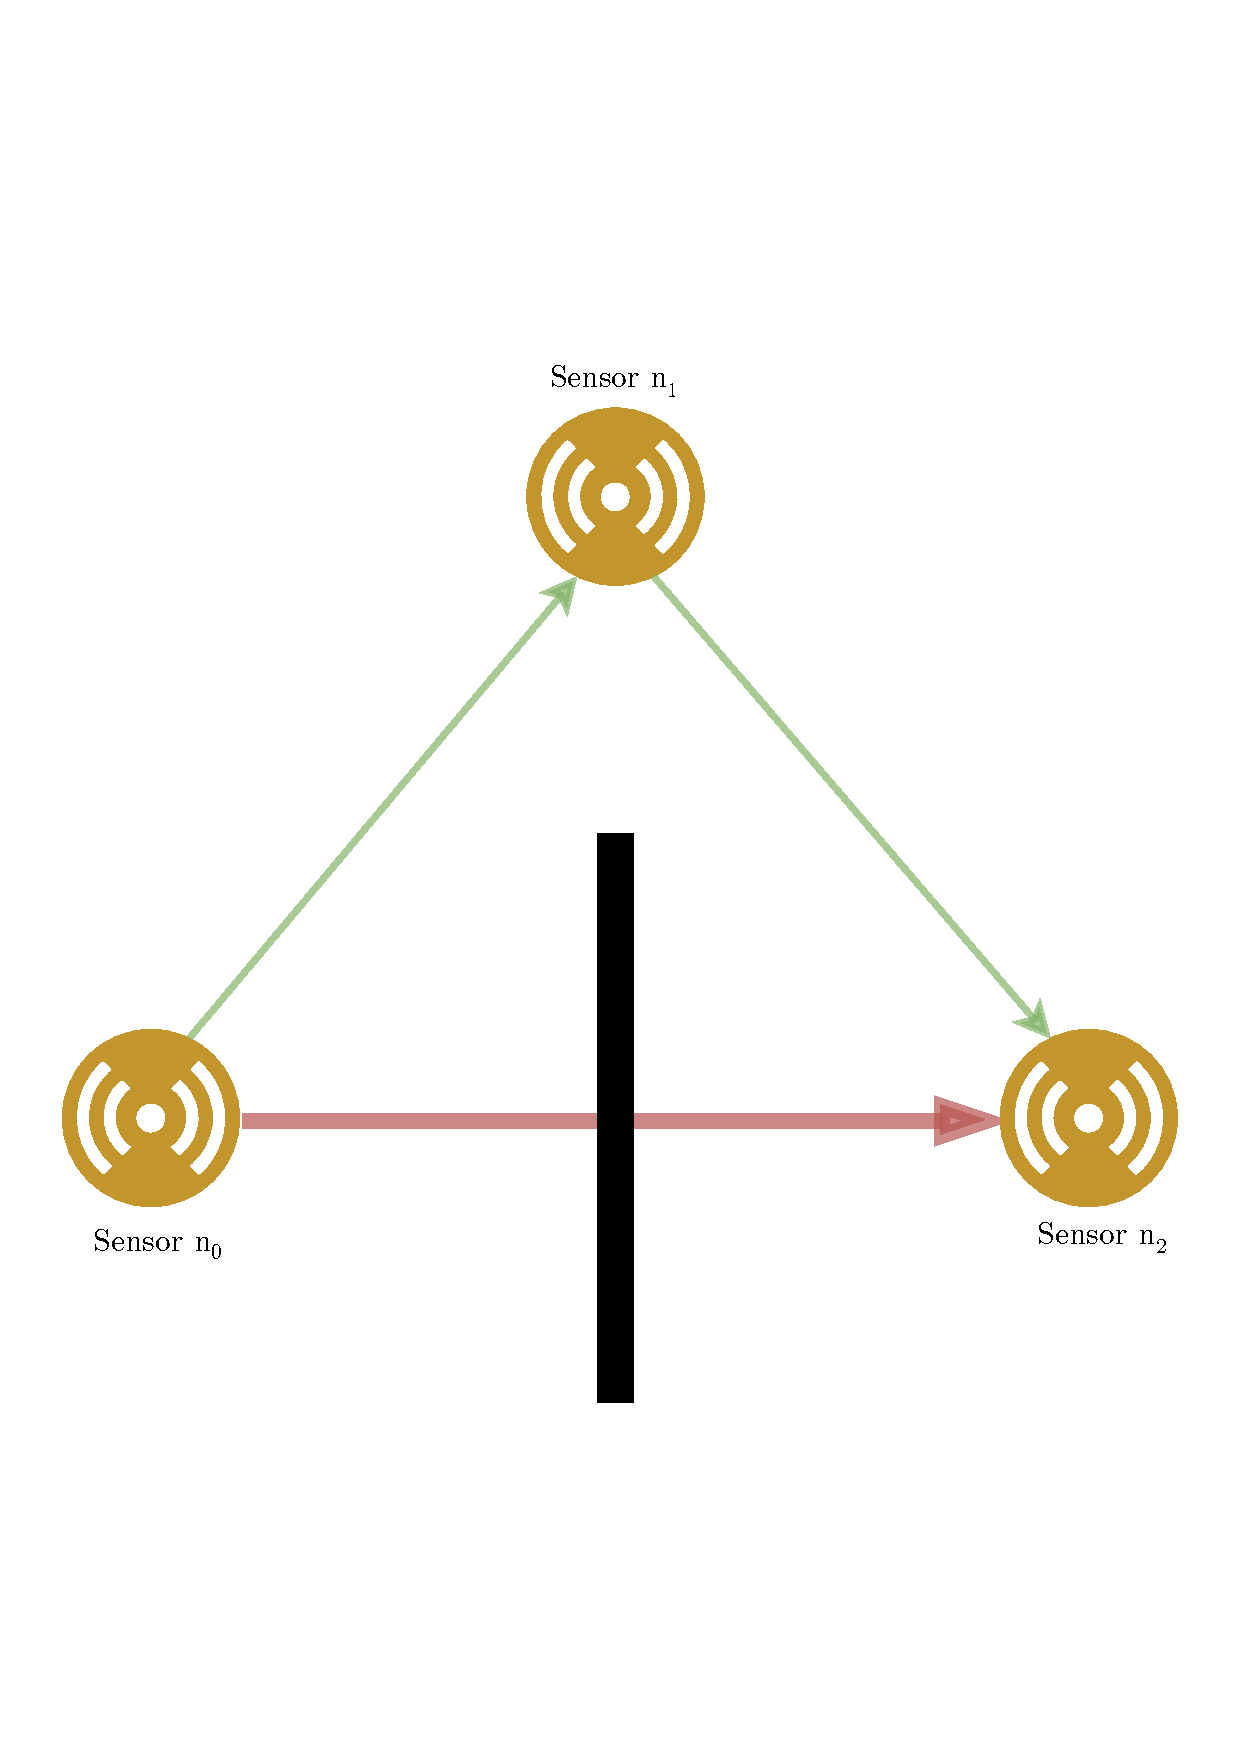
\includegraphics[width=0.7\linewidth]{resources/example3}
  \caption{Communication between three nodes in a wireless sensor network} \label{sensor_net}
\end{figure}
There are two possibilities for $n_0$. First, it can send directly the message to $n_2$. In that case, sending the message is quite quick, but requires more energy that a standard message sending. %(due to the demodulation of a noisy message by $n_2$).
Moreover, this sending has a risk of packet corruption due to the possible noise induced when the signal goes through the wall standing between the two sensors.
The second possibility is to send the message to an intermediate node (i.e., $n_1$). This sending is obviously slower due to the sending in two steps, but requires less energy in total that a direct sending.
In that case, the risk of packet corruption is negligible. \par
This example induces some questions. Firstly, we should be interested by a strategy ensuring a bounded duty cycle for the emitter sensor $n_0$ (i.e., a bounded time for its active session).
Thus, we should be interested by a strategy minimising the expected energy of sending the message while ensuring this duty cycle.
Finally, we should be interested by a strategy offering a good probability to have a bounded duty cycle while having a good probability to minimise the energy used by the sensor to send the message.
\end{example}
\section{Worst case guarantee}
Firstly, we are going to be interested in having a worst case guarantee to reach some states in a Markov decision process, i.e., a guarantee to reach these states with a cost bounded.
To do that, we approach the problem by considering it as a \textit{shortest path game} problem \cite{DBLP:journals/corr/RandourRS14a}.
\begin{definition}[\textbf{\SPG{} problem}]
  Let $\mathcal{M}$ be an MDP with state space $S$, $s \in S$, $T \subseteq S$, and $\ell \in \mathbb{N}$.
  The shortest path game problem (\SPG{}, for short) consists in deciding if there exists a strategy $\sigma$ ensuring to reach the subset of target states $T$ from the state $s$ with a cost bounded $\ell$, i.e.,
  \begin{align*}
    \forall \pi \in Paths^\sigma(s), \, \TS^T(\pi) \leq \ell.
  \end{align*}
\end{definition}

\begin{theorem}[\textbf{\textit{\SPG{} problem and qualitative cost bounded reachability}}] \label{spg-thm1}
  Let $\mathcal{M}=(S, A, \Delta, w, AP, L)$ be an MDP, $s \in S$, $T \subseteq S$, $\ell \in \mathbb{N}$, and $\sigma$ be a strategy for $\mathcal{M}$.
  The following two propositions are equivalent:
  \begin{enumerate}[(a)]
    \item $\forall \pi \in Paths^\sigma(s), \, \TS^T(\pi) \leq \ell$. \label{qsspp1}
    \item $\mathbb{P}_s^\sigma(\Diamond_{\leq \ell}\, T) = 1$. \label{qsspp2}
  \end{enumerate}
\end{theorem}
\begin{proof2}$ $\\
  ($\ref{qsspp1}\implies\ref{qsspp2}$). Assume that for any $\sigma$-path $\pi \in Paths^\sigma(s)$, the truncated sum of this path is lower than or equal to $\ell$, i.e., $\TS^T(\pi)\leq \ell$.
  We have $\mathbb{P}_s^\sigma(\Diamond_{\leq \ell}\, T) = \mathbb{P}_s^\sigma(\{ \pi \in Paths(s) \; | \; \TS^T(\pi) \leq \ell \})$. As all $\sigma$-paths starting from $s$ have a truncated sum lower than or equal to $\ell$, we have $\{\pi \in Paths^\sigma(s) \; | \; \TS^T(\pi) \leq \ell \} = Paths^\sigma(s)$.
  Then, $\mathbb{P}_s^\sigma(\Diamond_{\leq \ell}\, T) = \mathbb{P}_s^\sigma(Paths(s)) = 1$. \\
  ($\neg \ref{qsspp1} \implies \neg \ref{qsspp2}$). Assume there exists a $\sigma$-path $\pi \in Paths^\sigma(s)$ such that $\TS^T(\pi)>\ell$. Thus, consider this path $\pi$ and let $\hat{\pi} = s_0\xrightarrow{\alpha_1}\dots \xrightarrow{\alpha_n} s_n \in Pref(\pi)$, where $\alpha_i$ is
  chosen by the strategy $\sigma$ for each $i \in \{1, \dots, n \}$, such that $\sum_{i=1}^n w(\alpha_i) > \ell$.
  We have $\pi \in Cyl(\hat{\pi})$ and $\mathbb{P}_s^\sigma(Cyl(\hat{\pi})) = \prod_{i=0}^{n-1} \Delta(s_i, s_{i+1}) > 0$.
  We obviously additionally have that $Cyl(\hat{\pi}) \cap \{ \pi \in Paths^\sigma(s) \; | \; \TS^T(\pi) \leq \ell \} = \emptyset$, because %$s_i \not \in T$ for all $i \in \{0, \dots, n\}$ and
  %$\sum_{i=1}^n w(\alpha_i) > l$.
  $\TS^T(\hat{\pi}) > \ell$.
  Then, we have
   \[\mathbb{P}_s^\sigma(\Diamond_{\leq \ell}\, T) = \mathbb{P}_s^\sigma(\{ \pi \in Paths(s) \; | \; \TS^T \leq \ell \}) \leq 1 - \mathbb{P}_s^\sigma(Cyl(\hat{\pi})) < 1.\]
\end{proof2}
\\

Referring to Theorem \ref{spg-thm1}, it is possible to solve the \SPG{} problem by reduction to the \SSPP{} problem.
However, the \SSPP{} problem is computed in pseudo-polynomial time in $\mathcal{M}$ and in the size of the length of $\ell$, and we want to avoid this time complexity.
For this approach, we consider the MDP as a two players game.
In each step, the system is in state $s$ and the player one chooses an enabled action $\alpha$ of $s$.
Then, the player two chooses the $\alpha$-successor of $s$ leading the worst case in terms of truncated sum.
Thus, we do not consider probabilities for this problem but rather consider the worst case of choosing each action.
Finding an optimal strategy for the player one allowing to reach $T$ with a cost less than or equal to $\ell$
under the choices of the player two solves the \SPG{} problem. \\

We compute the shortest path in this game from $s$ to $T$ by dynamic programming in order to build a strategy satisfying the \SPG{} problem.
Let $|S| = n$ and $\mathbb{C}: S \times \{0, \dots, n-1 \}$ be a function such that $\mathbb{C}(s, i)$ is the shortest path from $s$ to $T$ after maximum
$i$ playing steps in this game.
Obviously, $\mathbb{C}$ can be represented with a matrix of size $n \times n$.
We have \[\mathbb{C}(s, 0) = \begin{cases}
  0 & \text{if } s \in T\\
  +\infty & \text{else}.
\end{cases}\]
Then, let $k \in \mathbb{N}$, such that $0 \leq k < n - 1$,
\[
  \mathbb{C}(s,\, k+1) = \min \big[\mathbb{C}(s,\, k),\, \min_{\alpha \in A(s)} \max_{s' \in Succ(s,\alpha)} \big(w(\alpha) + \mathbb{C}(s',\, k)\big)\big].
\]
This recursive definition of $\mathbb{C}$ actually means that the shortest path from $s$ to $T$ in maximum $k+1$ steps corresponds to either the shortest path from $s$ to $T$ in maximum $k$ steps or the minimal weight of choosing an action $\alpha$ plus the shortest path from the worst $\alpha$-successor $s'$ of $s$ to $T$ in maximum $k$ steps.
\begin{figure}[h]
  \centering
  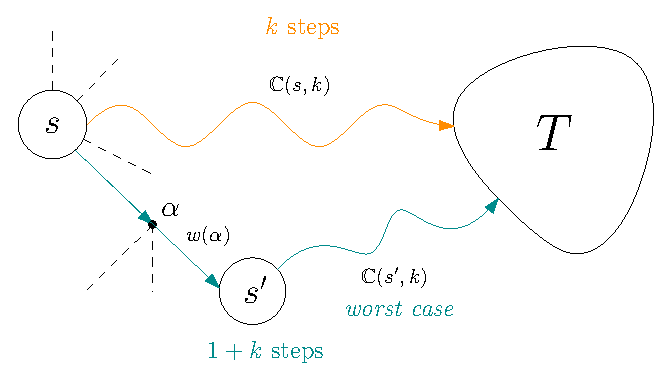
\includegraphics[width=0.6\linewidth]{resources/sp-g}
  \captionsetup{justification=centering}
  \caption{Intuitive representation of  the function $\mathbb{C}$, used to solve the \SPG{} problem}
\end{figure}
The minimisation term according to an action in this definition corresponds to the choice of the strategy (i.e., the player one).
The maximisation term in this definition corresponds to the adversary (i.e., the player two), choosing the worst $\alpha$-successor of $s$.
As the weight of each action is strictly positive, the strategy never chooses an action possibly leading to a  cycle in this game if it can avoid it.
Indeed, choosing an action possibly leading to a cycle necessarily yields an infinite truncated sum since the player two will necessarily choose the transition yiedling this cycle.
Thus, if a strategy satisfying this problem exists, it wins in at most $n$ steps. It is why we only need to consider the $n$ first steps.

\begin{theorem}[\textit{\textbf{Solving the \SPG{} problem}}] The \SPG{} problem can be decided in polynomial time in the size of $\mathcal{M}$, and % with the recursive function $\mathbb{C}$ (and more precisely in $\mathcal{O}(n^2)$ with memoization).
an optimal pure memoryless strategy always exists and can be built in polynomial time in the size of $\mathcal{M}$.
\end{theorem}
\begin{proof2}
By dynamic programming, we can determine the value of $\mathbb{C}$ for each entry $(s, i) \in S \times \{0, \dots, n-1\}$ with a time complexity in $\mathcal{O}(|S| \times |A|)$. This result corresponds to the worst case for which the set of enabled action of each state is $A$ and the set of $\alpha$-successor of this state is $S$, for each enabled action $\alpha$ (note that this case rarely happens in practice). Then, as $|S \times \{0, \dots, n-1\}| = |S|^2$, computing all values of $C$ for all entries $(s, i) \in S \times \{0, \dots, n-1\}$ can be done in $\mathcal{O}(|S|^3 \cdot |A|)$.
\par
Let $s$ be a state of the MDP. By definition of $\mathbb{C}$, we have $\mathbb{C}(s,\, k + 1) \leq \mathbb{C}(s,\, k)$, for all $k \in \mathbb{N}$ such that $0 \leq k < n-1$.
Then, we have $\mathbb{C}(s, \, n-1) = \min_{k} \mathbb{C}(s, \, k)$, and
a strategy satisfying the \SPG{} problem for $s \in S$ exists if and only if $\mathbb{C}(s,\, n-1) \leq \ell$.
Furthermore, we can build this pure memoryless strategy as follows:
\[
  \sigma : S \rightarrow A, \; s \mapsto \arg \min_{\alpha \in A(s)} \big[ \max_{s' \in Succ(s, \alpha)} \big(w(\alpha) + \mathbb{C}(s',\, n - 1) \big) \big].
\]
The key idea behind this definition is that $\sigma$ chooses the action minimising the weight of the enabled actions plus the smallest cost to reach $T$ in this game from the worst successor, chosen by the player two.

\end{proof2}
$ $\\

\begin{remark}[\textit{\SPG{} problem and PRCTL model checking}]
  Let $\mathcal{M}$ be an MDP with state space $S$ and atomic proposition space $AP$, $s \in S$, $\ell \in \mathbb{N}$, and $\Phi$ be a PRCTL state formula over $AP$,
  verify $s \models \mathcal{P}^{\max}_{=1}(\Diamond_{\leq \ell}\, \Phi)$ is equivalent to solve the \SPG{} problem for the state $s$, the cost threshold $\ell$, the subset of target states $Sat(\Phi)$ and the probability threshold one.
\end{remark}

\begin{example}[\textit{\SPG{} problem in the wireless sensor network}] \label{spg-example}
Getting back to Example \ref{main-example}, we will only consider the time dimension to model the situation of this example.
We focus on the behaviour of the node $n_0$  (cf. Figure \ref{sensor_net_mdp}).
When $n_0$ becomes active, it has to send a message to $n_2$. We assume here that a standard message sending takes $2$ \textit{mili seconds} ($ms$). If $n_0$ decides to send the message passing by $n_1$, it must wait to receive an acknowledgement of the message sent from $n_1$ to $n_2$. We assume that an acknowledgement message takes $2$ $ms$ to be received.
Thus, we have that $n_0$ sends the message to $n_1$ ($2$ $ms$), then $n_1$ sends the message to $n_2$ ($2$ $ms$). When $n_2$ receives the message, it sends an acknowledgement to $n_1$ ($2$ $ms$) and $n_1$ sends an acknowledgement to $n_0$ ($2$ $ms$).
Then, after that $n_0$ has sent the message to $n_1$, he waits $6$ $ms$ the acknowledgement from $n_1$ and go to sleep during $10$ $ms$ after that. If $n_0$ decides to directly send a message to $n_2$, then $n_2$ sends the message and waits $2$ $ms$ the acknowledgement.
Due to the possible packet corruption, $n_2$ does not receive the acknowledgement with a probability $\frac{1}{8}$. In that case, it has to try sending the message again.
Else, it goes to sleep during $10$ $ms$.
\begin{figure}[h]
  \centering
  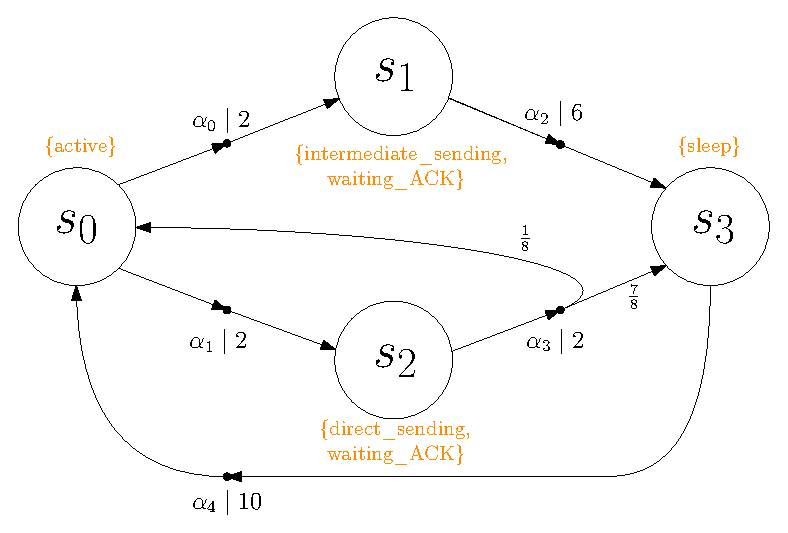
\includegraphics[width=0.6\linewidth]{resources/example3.eps}
  \captionsetup{justification=centering}
  \caption{MDP representing the behaviour of the node $n_0$, according to the situation of Figure \ref{sensor_net} from Example \ref{main-example}}\label{sensor_net_mdp}
\end{figure}

Assume we want to ensure a duty cycle of $12$ $ms$ for the node $n_0$. Then, let $\mathcal{M}=(S, A, \Delta, w, AP, L)$ be the MDP of Figure \ref{sensor_net_mdp}, we want to solve the following \SPG{} problem:
\[
  s_0 \overset{?}{\models} \, \mathcal{P}^{\max}_{=1}(\Diamond_{\leq 12} \; \textit{sleep}).
\]
To solve this problem, we will recursively compute $\mathbb{C}$ for all $s \in S$ from $k=0$ to $k=3$:\\[0.7em]
\begin{minipage}{0.5\linewidth}
    \begin{itemize}
      \item[$k=0$] \begin{itemize}
[label=\raisebox{0.25ex}{\tiny$\bullet$}]        \item $\mathbb{C}(s_0, 0) = \mathbb{C}(s_1, 0) = \mathbb{C}(s_2, 0) = +\infty$
        \item $\mathbb{C}(s_3, 0) = 0$
      \end{itemize}
      \item[$k=1$]
        \begin{itemize}
[label=\raisebox{0.25ex}{\tiny$\bullet$}]          \item $\mathbb{C}(s_0, 1) = +\infty$
          \item $\mathbb{C}(s_1, 1) = 6 + 0 = 6$
          \item $\mathbb{C}(s_2, 1) = 2 + \infty = +\infty$
        \end{itemize}
      \item[$k=2$]
        \begin{itemize}
[label=\raisebox{0.25ex}{\tiny$\bullet$}]          \item $\mathbb{C}(s_0, 2) = 2 + 6 = 8$
        \end{itemize}
      \item[$k=3$]
        \begin{itemize}
[label=\raisebox{0.25ex}{\tiny$\bullet$}]          \item $\mathbb{C}(s_2, 3) = 2 + 8 = 10$
        \end{itemize}
    \end{itemize}
\end{minipage}
\begin{minipage}{0.5\linewidth}
\centering
\begin{tabular}{l|llll}
$S$ & $k=0$     & $k=1$     & $k=2$     & $k=3$ \\ \hline
$s_0$  & $+\infty$ & $+\infty$ & 8         & 8     \\
$s_1$  & $+\infty$ & 6         & 6         & 6     \\
$s_2$  & $+\infty$ & $+\infty$ & $+\infty$ & 10    \\
$s_3$  & 0         & 0         & 0         & 0
\end{tabular}
\captionsetup{justification=centering}
\captionof{table}{Values of $\mathbb{C}$ (dynamic programming)}
\end{minipage}
\\$ $\\$ $\\
The result $\mathbb{C}(s_2,3)=10$ is interesting. It means that the player one firstly chooses the action $\alpha_3$ (with a weight of $2$).
Then, the player two chooses worst case, i.e., the transition $s_2 \xrightarrow{\alpha_3}s_0$, and the player one next chooses the action surely leading $s_0$ to $s_3$ with a minimal cost (i.e., $\mathbb{C}(s_0, 2)=8$ with $s_0\xrightarrow{\alpha_0}s_1\xrightarrow{\alpha_2}s_3$).
\par As $\mathbb{C}(s_0,\, 3) \leq 12$, the duty cycle is ensured by the strategy built with $\mathbb{C}$, and we have $s_0 \models \mathcal{P}^{\max}_{=1}(\Diamond_{\leq 12}\; \textit{sleep})$.
With this strategy, the sensor $n_0$ always chooses to send the message via $n_1$.
This ensures a duty cycle of $8$ $ms$, but it is possible to have a better expected time to reach the \textit{sleep} state while ensuring the dutty cycle of $12$ $ms$ (e.g., with a memory strategy).
So, the next type of strategy that we will study is strategies offering a good expected cost-to-target while ensuring to reach this target with a cost bounded.
\end{example}

\section{Good expectation under a worst case}
We now study strategies ensuring simultaneously a worst case guarantee (cf. previous section) and a good expected cost-to-target in a Markov decision process \cite{DBLP:journals/corr/RandourRS14a,DBLP:journals/corr/BruyereFRR13}.
\begin{definition}[\textbf{\SSPWE{} problem}]
    Let $\mathcal{M}$, be an MDP with state space $S$, $s \in S$, $T \subseteq S$, and $\ell_1, \ell_2 \in \mathbb{N}$.
    The \textit{stochastic shortest path worst case expectation} problem (\SSPWE{}, for short) consists in deciding if there exists a strategy $\sigma$ such that:
    \begin{itemize}
      \item $\forall \pi \in Paths^\sigma(s), \; TS^T(\pi) \leq \ell_1$.
      \item $\mathbb{E}_s^\sigma(\TS^T) \leq \ell_2$.
    \end{itemize}
\end{definition}

The \SSPWE{} problem is thus a \textit{multi-objective} problem: indeed, we actually want to solve simultaneously the \SPG{} problem and the \SSPE{} problem.
As a reminder, in the previous section we have replaced the probabilities by an adversarial choice to handle the guarantee to reach a set of target states according to a worst case.
Here, we will combine this approach with taking into account probabilities for the expected cost-to-target part.
Although the \SSPE{} and the \SPG{} problems can both be decided in polynomial time, the \SSPWE{} is more complex due to the strategy having to satisfy both problems at the same time.
%Before introducing an algorithm able to solve the problem, we first define the notion of \textit{attractor}.

\subsection{Attractors and dynamic programming}

In this subsection, we solve the problem by considering the unfolding of a given MDP $\mathcal{M}$ up to the worst case threshold $\ell_1$ and the set of target states $T$ as a game in order to ensure a worst case guarantee.
As for the \SPG{} problem, we thus consider at each turn that the player one chooses an enabled action $\alpha$ of a state, and that the player two chooses its $\alpha$-successor.
Before introducing an algorithm able to solve the \SSPWE{} problem, we first define the notion of \textit{attractor}.
\begin{definition}[\textbf{Attractor of a set of target states in an MDP}]
  Let $\mathcal{M}$ be an MDP with state space $S$ and $T \subseteq S$. The \textit{attractor} of $T$ is the set of states almost surely reaching $T$, i.e., the set $\Attr(T) = \{ s \in S \; | \; \mathbb{P}^{\max}_s (\Diamond T) = 1 \}$.
\end{definition}
Thus, an attractor is the set of states from which the player one can ensure to reach $T$ no matter what the player two does.
We restrict the state space of the unfolding of $\mathcal{M}$ to this attractor by computing the \textit{set of safe actions} for each state by dynamic programming, i.e., we compute the set of enabled actions of each state surely leading this state to a successor being in $\Attr(T)$.
We then compute the minimal expected cost-to-target in this MDP.
More formally, let $\mathcal{M}=(S, A, \Delta, w, AP, L)$ be an MDP, the \SSPWE{} problem for $\mathcal{M}$, the state $s \in S$, the subset of target states $T \subseteq S$, and the cost thresholds $\ell_1, \ell_2 \in \mathbb{N}$ can be solved with the following algorithm:

%\begin{center}
%  \hrule height.8pt depth0pt \kern2pt% \@fs@pre for \@fs@ruled
%  \captionof{algorithm}{Solving the \SSPWE{} problem}\label{sspwe-algo}
%  \vspace{-.02\linewidth}
%  \offinterlineskip\hrulefill
\begin{algorithm}[H]
\caption{Solving the \SSPWE{} problem}\label{sspwe-algo}
\begin{enumerate}
  \item We compute the unfolding of $\mathcal{M}$ from $s$ up to the cost threshold $\ell_1$, i.e., $\mathcal{M}_{\ell_1}$ with state space $S_{\ell_1}$.
  %\item We compute $\mathbb{A}: S \times \{0, \dots, \ell_1\} \cup \{\bot\} \rightarrow A$, for each state of $S_{\ell_1}$, yielding the set of \textit{safe actions} allowing to surely go to a successor being in the attractor of $T_{\ell_1} = \{ (s, v) \in S_{\ell_1} \; | \; s \in T \, \wedge \, v \leq \ell_1 \}$.
  \item Then, we compute the set of \textit{safe actions} allowing each state in $S_{\ell_1}$ to surely go to a successor being in the attractor of
  $T_{\ell_1} = \{ (s, v) \in S_{\ell_1} \; | \; s \in T \, \wedge \, v \leq \ell_1 \}$, whatever the action chosen in this set by any strategy for $\mathcal{M}_{\ell_1}$.
  More formally, we compute $\mathbb{A}: S_{\ell_1} \rightarrow 2^A$, \[ (s, v) \mapsto \{ \alpha \in A(s) \; | \; \forall (s', v') \in Succ((s, v), \, \alpha), \, (s', v') \in \Attr(T_{\ell_1}) \}\]
  for all states $(s, v) \in S_{\ell_1}$. Thus, for each state $(s, v) \in S_{\ell_1}$, $\mathbb{A}(s, v)$
  is the set of actions $\alpha \in A(s)$ ensuring to almost surely reach $T_{\ell_1}$ from $(s, v)$.
  \item Next, we compute $\mathcal{M}^\mathbb{A}_{\ell_1}$, the unfolding of $\mathcal{M}$ up to $\ell_1$ restricted by the attractor of $T_{\ell_1}$. The key idea is that we remove the states $(s, v)$ such that $\mathbb{A}(s, v) = \emptyset$ from $\mathcal{M}_{\ell_1}$. More formally,
  we define $\mathcal{M}^\mathbb{A}_{\ell_1} = (S^\mathbb{A}_{\ell_1}, \mathbb{A}^*, \Delta^*_{\ell_1}, w, AP, L_{\ell_1})$ as follows:
  \begin{itemize}
    \item $S^\mathbb{A}_{\ell_1} = \{ (s, v) \in S_{\ell_1} \; | \; \mathbb{A}(s, v) \neq \emptyset \, \vee \, (s, v) \in T_{\ell_1} \}$,
    \item $\mathbb{A}^*$ is the set of action of this unfolding such that, for all action $\alpha \in A$, $\alpha \in \mathbb{A}^*$, and the set of enabled actions of each state $(s, v) \in S^\mathbb{A}_{\ell_1}$ is given by %$\mathbb{A}(s, v)$ if $\mathbb{A}(s, v) \neq \emptyset$ and a singleton containing an arbitrary action $\alpha \in A(s)$ else,
    \[
      \mathbb{A}^*(s, v) = \begin{cases}
        \mathbb{A}(s, v) & \text{if } \mathbb{A}(s, v) \neq \emptyset, \, \\
        \{\alpha\}, \; \text{where } \alpha \in A(s) & \text{else},
      \end{cases}
    \]
    \item $\Delta^*_{\ell_1}$ is defined the same way as for the classical unfolding $\mathcal{M}_{\ell_1}$, except for $(s, v)$ such that $\mathbb{A}(s, v) = \emptyset$, where $\Delta^*_{\ell_1}((s, v),\, \alpha, \, (s, v)) = 1$ and $\Delta^*_{\ell_1}((s, v), \, \alpha, \, (s', v')) = 0$ if $(s', v') \neq (s, v)$, for $\alpha \in \mathbb{A}^*(s, v)$.
    \item $L_{\ell_1}$ is defined as for the classical unfolding $\mathcal{M}_{\ell_1}$.
  \end{itemize}
  Note that we define $\mathbb{A}^*$ and $\Delta_{\ell_1}^*$ this way because we must handle the case of $(s, v) \in T_{\ell_1}$ and $\mathbb{A}(s, v) = \emptyset$.
  \item Finally, we solve the \SSPE{} problem in $\mathcal{M}^\mathbb{A}_{\ell_1}$ for the state $(s, 0)$, the subset of target states $T_{\ell_1}$, and the cost threshold $\ell_2$.
\end{enumerate}
\end{algorithm}
%$ $\\
%\kern2pt\hrule\relax% \@fs@post for \@fs@ruled
%\end{center}
%\par
Let $(s, v) \in S_{\ell_1}$, the set of safe actions of $(s, v)$, i.e., $\mathbb{A}(s, v)$, can be computed recursively
% with the function $\mathbb{A}_i$, for $i \in \mathbb{N}$, %corresponding to the set of actions ensuring to reach a \textit{safe state} in $i$ steps (i.e., a state in the attractor of $T_{\ell_1}$),
%that is defined
as follows:
\begin{equation}
  \mathbb{A}_0(s, v) = \begin{cases}
    A(s) & \text{if }v \leq \ell_1,\\
    \emptyset & \text{else}.
  \end{cases} \label{attractor-set-init}
\end{equation}
Then, let $i \in \mathbb{N}$, assume that $\mathbb{A}_i$ has already been computed,
\begin{equation}
  \mathbb{A}_{i+1}(s, v) = \{ \alpha \in \mathbb{A}_i(s, v) \; | \;
    \forall (s', v') \in Succ( (s, v), \alpha ) \setminus T_{\ell_1}, \; \mathbb{A}_i(s', v') \neq \emptyset \}.
    \label{attractor-set}
\end{equation}
%The key idea behind this definition is that
%$\mathbb{A}_i(s,v)$ is the set of enabled actions of $(s, v)$ ensuring to not reach a \textit{bad state} in at most $i$ transitions.
The key idea behind this definition of $\mathbb{A}_i$ is that we inductively disable the unsafe enabled actions of all states.
We consider that a state that has no more enabled action is a \textit{bad state}.
At the initialisation, i.e., at $i=0$, all enabled actions of each state are safe except if the current cost of a state has exceeded the threshold $\ell_1$. In that case, this state is a bad state.
%Then, we inductively consider the successors  of $(s, v)$ reachable in $i$ steps from the current state $(s, v)$ and inductively remove the enabled actions of $(s, v)$ ensuring to reach a bad states from one of these successors, in at most $i$ steps.
%Then, we inductively increase the scope of successors considered up to a \textit{bad state}, i.e., a state exceeding the cost $\ell_1$. Each action
By induction on $i$, at each step and for each state $(s, v)$,
%By induction, at the step $i$,
we disable the actions $\alpha$
%of each state
that risk to lead $(s, v)$ to one of its $\alpha$-successor considered as a bad state.% in at most $i$ transitions.
\begin{figure}[h]
  \begin{minipage}{0.5\linewidth}
    \centering
    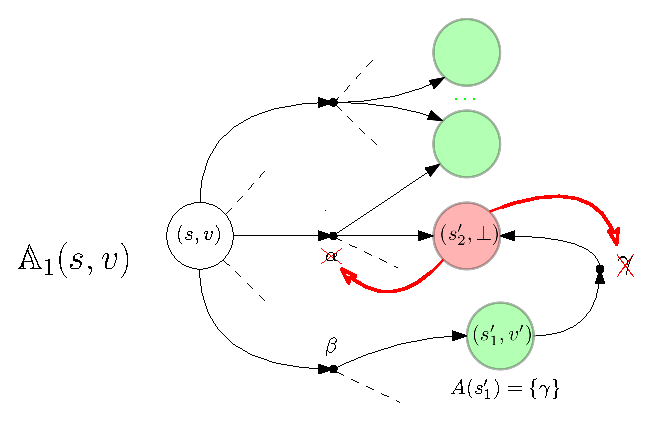
\includegraphics[width=0.9\linewidth]{resources/attractor}
  \end{minipage}
  \begin{minipage}{0.5\linewidth}
    \centering
    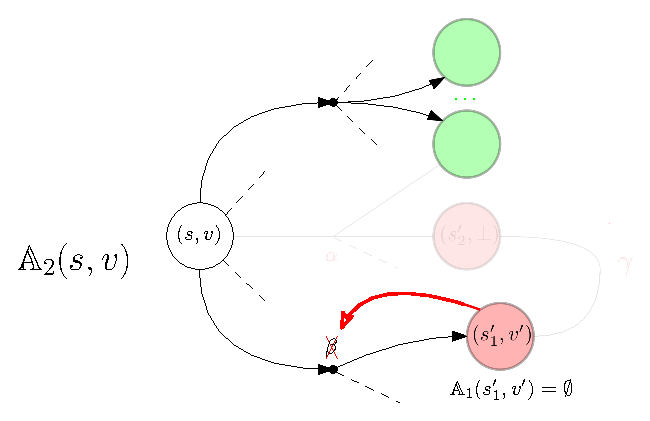
\includegraphics[width=0.9\linewidth]{resources/attractor2}
  \end{minipage}
  \caption{Intuition of the recursive computation of $\mathbb{A}$}
\end{figure}
%The way we compute $\mathbb{A}$ is actually an adaptation of the method used to compute the largest set $S_{=1} = \{ s \in S \; | \; \mathbb{P}^{\max}_s(\Diamond T) = 1 \}$ (cf. Algorithm \ref{prMax1} from Subsection \ref{temp-event-mdp}).
%Computing $\mathbb{A}$ this way actually particularises Algorithm \ref{prMax1} for $\mathcal{M}_{\ell_1}$ and rather return actions leading to attractors of $T_{\ell_1}$, in order to build $\mathcal{M}^\mathbb{A}_{\ell_1}$ and solve the \SSPE{} problem in it.

\noindent Inspired by Algorithm \ref{prMax1} from Subsection \ref{temp-event-mdp}, we build a matrix $\mathbb{A}$ with algorithm \ref{safe-actions-algorithm}.

\begin{algorithm}[H]
\caption{Computing the matrix of safe actions $\mathbb{A}$}
\label{safe-actions-algorithm}
\begin{algorithmic}[1]
\REQUIRE{
		$\mathcal{M}_{\ell_1} = (S_{\ell_1}, A_{\ell_1}, \Delta, w, AP, L)$, the unfolding of an MDP $\mathcal{M}$ up to $\ell_1$, and
		$T_{\ell_1} \subseteq S$, a subset of target states in this unfolding.
	}
\ENSURE{
	The safe action matrix $\mathbb{A}$
}
\STATE $\mathbb{A} \leftarrow $ {\sffamily initialise} a matrix of size $|S| \times \ell_1$ with $\emptyset$ \label{attr1}
\FOR{$(s, v) \in S_{\ell_1} \setminus \{s_\bot\}$}
  \STATE $\mathbb{A}(s, v) \leftarrow A_{\ell_1}(s, v)$ \label{attr3}
\ENDFOR
\STATE $U \gets \{ s_\bot \}$ \label{attr4}
\COMMENT{$U$ is the set of ``bad states''}
\WHILE{$U \neq \emptyset$}
	\STATE $R \gets U$ \label{attr5}
	\WHILE{$R \neq \emptyset$}\label{attr13}
		\STATE {\sffamily let} $(s', v') \in R$
		\COMMENT{let $(s', v')$ be a bad state of $\mathcal{M}_{\ell_1}$}
		\STATE $U \gets U \setminus \{(s', v') \}$ \label{attr6}
		\STATE $R \gets R \setminus \{(s', v') \}$\label{attr7}
		\COMMENT{``mark'' $(s', v')$ as visited}
    \IF{$(s', v') \not\in T_{\ell_1}$}
  		\FORALL{$((s, v), \alpha) \in Pred((s', v'))$ such that $\alpha \in \mathbb{A}(s, v)$} \label{attr8}
  			\STATE $\mathbb{A}(s, v) \leftarrow \mathbb{A}(s, v) \setminus \alpha$\label{attr9}
  			\IF{$\mathbb{A}(s, v) = \emptyset$}
  				\STATE $U \gets U \cup \{ (s, v) \}$ \label{attr10}
  			\ENDIF
  		\ENDFOR
		\ENDIF
		%\STATE remove $u$ and its outgoing edges in $\mathcal{M}$
	\ENDWHILE
\ENDWHILE
\RETURN $\mathbb{A}$
\end{algorithmic}
\end{algorithm}


\begin{lemma}[Correctness of Algorithm \ref{safe-actions-algorithm}]
  Algorithm \ref{safe-actions-algorithm} is exact and computes $\mathbb{A}$.
\end{lemma}

\begin{proof2}
The construction of $\mathbb{A}$ by Algorithm \ref{safe-actions-algorithm} exactly behaves like the recursive computation of $\mathbb{A}$, but allows to only consider the interesting states at each step instead of always checking all states of the system.
The key idea behind this algorithm is that we remember at each iteration $i$ which states $(s',v')$ become bad states, in order to remove at iteration $i+1$ all enabled actions $\alpha$ from each state $(s, v)$ such that a bad state $(s', v')$ is in the set of $\alpha$-successors of $(s, v)$. \\
More formally, we prove that $\mathbb{A}$ is equal to $\mathbb{A}_i$ at each iteration $i$ of the algorithm.
\par At the initialisation, i.e., at $i=0$,
we initialise $\mathbb{A}$ with $\{s_\bot\}$ (lines \ref{attr1} to \ref{attr3}), what exactly agrees with $\mathbb{A}_0$ (cf. Equation \ref{attractor-set-init}).
Indeed, by definition of $\mathcal{M}_{\ell_1}$, being the unfolding of $\mathcal{M}$ up to $\ell_1$, the state $s_\bot$ exactly captures all the states for which the threshold $\ell_1$ have been exceeded.
Note that we additionally initialise a variable $U$ with $\{s_\bot\}$ (line \ref{attr4}).\\
Then, let $i \in \mathbb{N}_0$, we assume that $\mathbb{A}(s, v) = \mathbb{A}_i(s, v)$ for all states $(s, v) \in S_{\ell_1}$ at iteration $i$.
Moreover, we assume that all bad states $(s', v')$ of $\mathbb{A}_i$ such that $\mathbb{A}_i(s', v')=\emptyset$ are strictly in $U$ at iteration $i$, i.e., \[U = U_i = \{(s', v') \in S_{\ell_1} \; | \; \mathbb{A}_i(s', v') = \emptyset \; \wedge \; \mathbb{A}_{i-1}(s', v') \neq \emptyset \}.\]
We are going to proof that $\mathbb{A}(s, v) = \mathbb{A}_{i+1}(s, v)$ and that $U = U_{i+1}$ at the end of the iteration $i+1$.\\
Let $R$ be a new set strictly containing all states of $U_i$ (line \ref{attr5}).
For all bad states $(s', v')$ of $R$, we start by removing $(s', v')$ from $U$ and $R$ (lines \ref{attr6} and \ref{attr7}).  {\color{umons-red}(*)}\\
For each predecessor of each state removed from $U$, i.e., for each $((s, v), \alpha) \in Pred((s', v'))$ such that $(s', v') \not \in T_{\ell_1}$ and $\alpha \in \mathbb{A}(s, v)$, we remove $\alpha$ from $\mathbb{A}(s, v)$, i.e., we remove each action $\alpha \in \mathbb{A}(s, v)$ such that there is a bad state $(s', v') \in Succ((s, v), \alpha) \setminus T_{\ell_1}$, where $\mathbb{A}_i(s', v') = \emptyset$
(lines \ref{attr8} and \ref{attr9}).
 {\color{umons-red}(**)}\\
Finally, following this modification of $\mathbb{A}$, if $\mathbb{A}(s, v) = \emptyset$, we add $(s, v)$ in $U$ (line \ref{attr10}). {\color{umons-red}(***)}\\
First, by {\color{umons-red}(**)}, we exactly have that $\mathbb{A}(s, v) = \mathbb{A}_{i+1}(s, v)$, for all $(s, v) \in S_{\ell_1}$ (cf. Equation \ref{attractor-set}). Indeed, at iteration $i+1$, \[\mathbb{A}(s, v) = \mathbb{A}_{i}(s, v) \setminus
\{ \alpha \in \mathbb{A}_{i}(s, v) \; | \; \forall (s', v') \in Succ((s, v), \alpha) \setminus T_{\ell_1}, \, (s', v') \in U_i\},\]
for all $(s, v) \in S_{\ell_1}$.\\
By {\color{umons-red}(*)}, when $R$ is empty (line \ref{attr13}), all bad states of $U_i$ have been considered, i.e., we have removed each state $(s', v')$ such that $\mathbb{A}_{i}(s, v) = \emptyset$ from $U$.
Then, by {\color{umons-red}(***)}, we have that $U$ equals to $U_{i+1} = \{(s', v') \in S_{\ell_1} \; | \; \mathbb{A}_{i+1}(s', v') = \emptyset \; \wedge \; \mathbb{A}_{i}(s', v') \neq \emptyset  \}$.

\end{proof2}

\begin{theorem}[\textbf{\textit{Solving the \SSPWE{} problem}}]
  The \SSPWE{} problem can be decided in pseudo-polynomial time in the size of $\mathcal{M}$ and in the size of the length of $\ell_1$.
  Pure pseudo-polynomial memory strategies are sufficient and in general necessary, and strategies satisfying this problem can be built in pseudo-polynomial time in the size of $\mathcal{M}$ and in the size of the length of $\ell_1$.
\end{theorem}

By definition, the size of the set $\mathbb{A}_i$ is decreasing with $i$, i.e., for all $i \in \mathbb{N}$,
\[
  | \mathbb{A}_i | \geq | \mathbb{A}_{i+1} |.
\]
%By construction, the underlying graph of the unfolding of $\mathcal{M}$ up to $\ell_1$ is a directed acyclic graph (i.e., a DAG). Indeed, the weight of each action is a strictly positive integer. Then, there is no cycle in $\mathcal{M}_{\ell_1}$ and each state reach $T_{\ell_1}$ in at most $\ell_1$ transitions (this worst case corresponds to the case of $w(\alpha)=1$ for all $\alpha \in A$).
The time complexity of the construction of $\mathbb{A}$ is polynomial in the size of $\mathcal{M}_{\ell_1}$, and is thus pseudo-polynomial in the size of $\mathcal{M}$ and in the length of $\ell_1$.
So, as solving the \SSPE{} problem in $\mathcal{M}^\mathbb{A}_{\ell_1}$ is polynomial in the size of $\mathcal{M}^\mathbb{A}_{\ell_1}$,
the entire algorithm presented to solve this problem is pseudo-polynomial in the size of $\mathcal{M}$ and in the size of the length of $\ell_1$.
Furthermore, as the strategy solving the \SSPE{} problem in $\mathcal{M}_{\ell_1}^\mathbb{A}$ is memoryless in $\mathcal{M}_{\ell_1}^\mathbb{A}$, it requires pseudo-polynomial memory in $\mathcal{M}$ (intuitively, the strategy has $\ell_1 + 1$ modes).

\begin{example}[\textit{\SSPWE{} problem in the wireless sensor network}]
  Again, we get back to Example \ref{main-example}.
  We consider the MDP $\mathcal{M}$ of Figure \ref{sensor_net_mdp}. As in Example \ref{spg-example}, we are interested by a strategy ensuring a duty cycle of $12$ $ms$ for the node $n_0$, but at the same time ensuring a minimal expected time to reach the \textit{sleep} state, allowing it to go to sleep as soon as possible.
  Assume that we are interested by the following \SSPWE{} problem:
  \[
    ?\exists \sigma \; \;  \mathbb{P}^\sigma_{s_0}(\Diamond \{s_2\}) \leq 12 \; \wedge \; \mathbb{E}^\sigma_{s_0}(\TS^{\{s_2\}}) \leq 6,
  \]
  where $6$ $ms$ is half the time of the duty cycle that we want to ensure. First, we begin by unfolding $\mathcal{M}$ from $s_0$ up to the cost threshold $\ell_1 = 12$ (cf. Figure \ref{unfolding-sspwe}), yielding the MDP $\mathcal{M}_{\ell_1}$.
  \begin{figure}[h]
    \centering
    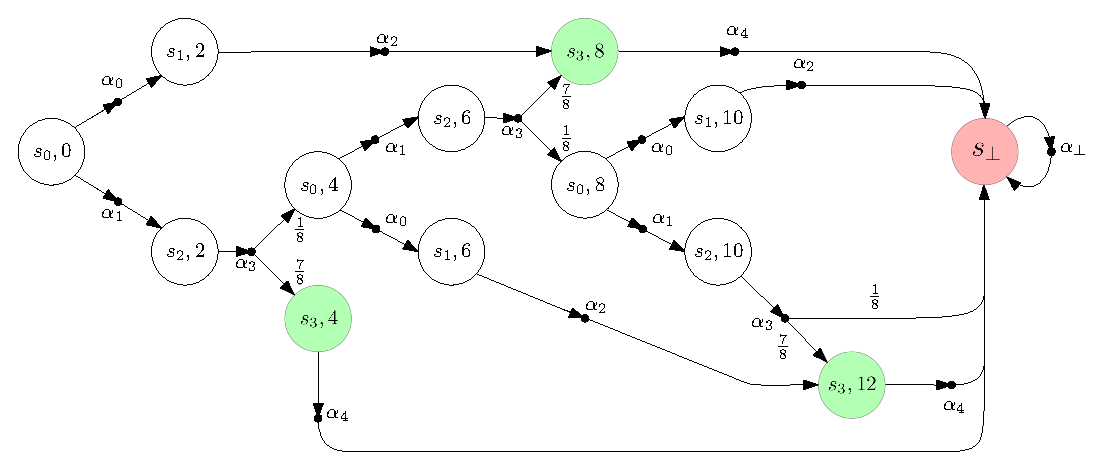
\includegraphics[width=0.9\linewidth]{resources/main-example-unfolding}
    \captionsetup{justification=centering}
    \caption{Unfolding of $\mathcal{M}$ (cf. Figure \ref{sensor_net_mdp}) from $s_0$ (i.e., from the active state) up to $12$ $ms$}
    \label{unfolding-sspwe}
  \end{figure}
  \begin{table}[h]
  \centering
\begin{tabular}{l|cccccc}
$S_{\ell_1}$          & \multicolumn{1}{l}{$i=0$} & \multicolumn{1}{l}{$i=1$}                                  & \multicolumn{1}{l}{$i=2$}  & \multicolumn{1}{l}{$i=3$}  & \multicolumn{1}{l}{$i=4$} & \multicolumn{1}{l}{$i=5$} \\ \hline
$s_0, \, 0$  & $\alpha_0, \alpha_1$      & $\alpha_0, \alpha_1$                                       & $\alpha_0, \alpha_1$       & $\alpha_0, \alpha_1$       & $\alpha_0, \alpha_1$      & $\alpha_0, \alpha_1$      \\
$s_1, \, 2$  & $\alpha_2$                & $\alpha_2$                                                 & $\alpha_2$                 & $\alpha_2$                 & $\alpha_2$                & $\alpha_2$                \\
$s_2, \, 2$  & $\alpha_3$                & $\alpha_3$                                                 & $\alpha_3$                 & $\alpha_3$                 & $\alpha_3$                & $\alpha_3$                \\
$s_0, \, 4$  & $\alpha_1, \alpha_0$      & $\alpha_1, \alpha_0$                                       & $\alpha_1, \alpha_0$       & $\alpha_1, \alpha_0$       & ${\color{red}\alpha_0}$   & $\alpha_0$                \\
$s_3, \, 4$  & $\alpha_4$                & ${\color{red}\varnothing}$                                 & $\varnothing$              & $\varnothing$              & $\varnothing$             & $\varnothing$             \\
$s_1, \, 6$  & $\alpha_2$                & $\alpha_2$                                                 & $\alpha_2$                 & $\alpha_2$                 & $\alpha_2$                & $\alpha_2$                \\
$s_2, \, 6$  & $\alpha_3$                & $\alpha_3$                                                 & $\alpha_3$                 & ${\color{red}\varnothing}$ & $\varnothing$             & $\varnothing$             \\
$s_0, \, 8$  & $\alpha_0, \alpha_1$      & $\alpha_0, \alpha_1$                                       & ${\color{red}\varnothing}$ & $\varnothing$              & $\varnothing$             & $\varnothing$             \\
$s_3, \, 8$  & $\alpha_4$                & ${\color{red}\varnothing}$                                 & $\varnothing$              & $\varnothing$              & $\varnothing$             & $\varnothing$             \\
$s_1, \, 10$ & $\alpha_2$                & ${\color{red}\varnothing}$                                 & $\varnothing$              & $\varnothing$              & $\varnothing$             & $\varnothing$             \\
$s_2, \, 10$ & $\alpha_3$                & ${\color{red}\varnothing}$                                 & $\varnothing$              & $\varnothing$              & $\varnothing$             & $\varnothing$             \\
$s_3, \, 12$ & $\alpha_4$                & ${\color{red}\varnothing}$ & $\varnothing$              & $\varnothing$              & $\varnothing$             & $\varnothing$             \\
$s_\bot$     & $\varnothing$             & $\varnothing$                                              & $\varnothing$              & $\varnothing$              & $\varnothing$             & $\varnothing$
\end{tabular}
  \caption{Computation of $\mathbb{A}_i$ by dynamic programming}
  \label{my-table2}
\end{table}
Then, we compute iteratively $\mathbb{A}_i$ until reaching an index $i^*$ such that $\mathbb{A}_{i^*} = \mathbb{A}_{i^*+1}$ (all sets $\mathbb{A}_{j}(s, v)$ such that $j \geq i^*$ are equal to $\mathbb{A}_{i^*}(s, v)$ for $(s, v)\in S_{\ell_1}$), and we thus have $\mathbb{A} = \mathbb{A}_{i^*}$.
In our case, we compute $\mathbb{A}_i$ by dynamic programming (cf. Table \ref{my-table2}), and we see that $\mathbb{A}_4=\mathbb{A}_5$. Thus, we have $\mathbb{A} = \mathbb{A}_4$.
Finally, we limit $\mathcal{M}_{\ell_1}$ to the safe actions of $\mathbb{A}$, yielding the MDP $\mathcal{M}_{\ell_1}^\mathbb{A}$ (cf. Figure \ref{safe_actions}).
We solve the \SSPE{} problem in $\mathcal{M}_{\ell_1}^\mathbb{A}$ for $s_0$, the set of target states $T_{\ell_1} = \{(s_3, 4), \, (s_3, 8), \, (s_3, 12)\}$, and the cost threshold $\ell_2 = 6$.
\begin{figure}[h!]
  \centering
  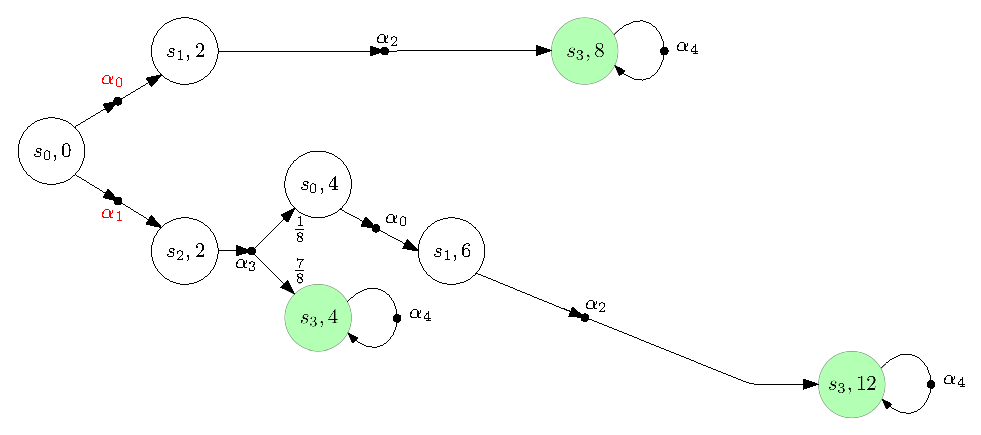
\includegraphics[width=0.8\linewidth]{resources/main-example-unfoldingA}
  \caption{$\mathcal{M}_{\ell_1}$ limited to safe actions of $\mathbb{A}$}
  \label{safe_actions}
\end{figure}
In $\mathcal{M}_{\ell_1}^\mathbb{A}$, we can easily compute the minimal expected cost-to-target for $T_{\ell_1}$ since there is actually only one nondeterministical choice: either the strategy chooses $\alpha_0$ for the state $(s_0, 0)$ and the expected cost-to-target corresponding to this choice is $8$, or it chooses $\alpha_1$ (we denote this strategy $\sigma_{\alpha_1}$), and the expected cost-to-target is
\[
  \mathbb{E}^{\sigma_{\alpha_1}}_{(s_0, 0)}(\TS^{T_{\ell_1}}) = \frac{7}{8} \cdot 4 + \frac{1}{8} \cdot 12 = 5.
\]
Thus, the minimal expected cost from $s$ to $T$ while ensuring to reach $T$ with probability one is $5 \leq 6$, and thus the \SSPWE{} problem is solved. The optimal pure memoryless strategy $\sigma_{\alpha_1}$ in $\mathcal{M}_{\ell_1}^\mathbb{A}$ corresponds
in $\mathcal{M}$ to the memory strategy trying once $\alpha_1$, and then choosing $\alpha_0$ if it has failed, i.e., trying once a direct sending to the node $n_2$, and then sending the message via the intermediate node $n_1$ if it has failed.
\end{example}

\section{Multi-objective reachability}
\label{mosr-section}
Now, we interest us in strategies satisfying simultaneously multiple reachability problems.
The problem consisting in deciding the existence of
such a strategy is the \textit{multi-objective stochastic reachability} \cite{DBLP:journals/lmcs/EtessamiKVY08}.
In order to know if we can define a strategy satisfying simultaneously $n$ reachability problems with given probabilities, we interest us in the simultaneously \textit{achievable} vectors $(p_1, \dots, p_n)$ of probabilities for these problems, i.e., such that there exists a strategy ensuring the reachability problem $i$ with a probability $p_i$ for all $i \in \{1, \dots, n\}$.
Furthermore, we interest us in the ``trade-off" curve, named \textit{Pareto curve}, being the set of optimal achievable vectors.
Indeed, there can be some compromises between different reachability properties. For instance,
assume we define a strategy ensuring the reachability to two set of target states $T_1$ and $T_2$ with probabilities $(p_1, p_2)$.
 Modify the strategy to increase the probability $p_1$ of reaching the set $T_1$ may necessitate to lower the probability $p_2$ of reaching the set $T_2$.

\begin{definition}[\textbf{Multi-objective stochastic reachability problem}]
  Let $\mathcal{M}$ be an MDP with state space $S$, action space $A$, and probability transition function $\Delta$, $s \in S$, and $r \in \mathbb{N}$ reachability properties.
  These properties are described by a set of target states $T_i \subseteq S$, and the probability threshold $\alpha_i \in [0, 1] \cap \mathbb{Q}$, for each $i \in \{1, \dots, r\}$.
  The \textit{multi-objective stochastic reachability} problem (\MOSR{}, for short) consists in deciding if there exists a strategy $\sigma$ satisfying
  \[
    \bigwedge_{i=1}^r \mathbb{P}^\sigma_s(\Diamond T_i) \geq \alpha_i.
  \]
\end{definition}


\subsection{Pareto curve}
We now define formally what are achievable vectors for a given \MOSR{} problem and what is the Pareto curve associated.
We actually need these notions to introduce the resolution of all \MOSR{} problems.
Indeed, solving such a problem requires to investigate a multi-objective optimisation problem that is highly linked to this Pareto curve.\\

Let $\mathcal{M}$ be an MDP with state space $S$, action space $A$, and transition probability function $\Delta$, and
$
  \mathcal{Q}_{s, r} := \,?\exists \sigma\; \bigwedge_{i=1}^r \mathbb{P}^\sigma_s(\Diamond T_i) \geq \alpha_i
$
be a \MOSR{} problem for $s \in S$, $r \in \mathbb{N}$, $(T_i)_{i \in \{1, \dots, r\}} \subseteq S^r$, and $\alpha \in ([0, 1] \cap \mathbb{Q})^r$.

\begin{definition}[\textbf{Achievable vectors}]
An \textit{achievable vector of $\mathcal{Q}_{s, r}$} is a vector $(p_i)_{i \in \{1, \dots, r\}}$ such that there exists a strategy $\sigma$ for $\mathcal{M}$ where $p_i = \mathbb{P}^\sigma_s(\Diamond T_i) \geq \alpha_i$ for all $i \in \{1, \dots, r\}$.
Furthermore, the \textit{achievable set of $\mathcal{Q}_{s, r}$} is given by
\[U_{\mathcal{Q}_{s, r}} = \{ \, p \in ([0, 1]) \cap \mathbb{Q})^r \; | \; \exists \sigma, \; p = (\mathbb{P}_s^\sigma (\Diamond T_i))_{i \in \{1, \dots, r\}} \, \}\]
\end{definition}

\begin{definition}[\textbf{Pareto optimal vector}]
  Let $p \in U_{\mathcal{Q}_{s, r}}$ be an achievable vector of $\mathcal{Q}_{s, r}$.
  This vector $p$ is \textit{Pareto optimal} if and only if there does not exists another vector domininating $p$, i.e., $\neg \exists p' \in U_{\mathcal{Q}_{s, r}}$ such that $p \leq p'$ and $p \neq p'$
  (where $\leq$ is the coordinate-wise inequality, i.e., $p\leq p'$ if and only if $p_i \leq p'_i$, for all $i \in \{1, \dots, r\}$).
\end{definition}

\begin{definition}[\textbf{Pareto curve}]
  The \textit{Pareto curve} $\mathpzc{P}_{\mathcal{Q}_{s, r}}$
  of the \MOSR{} problem $\mathcal{Q}_{s, r}$ is the set of Pareto optimal vectors inside $U_{\mathcal{Q}_{s, r}}$, i.e.,
  \[
    \mathpzc{P}_{\mathcal{Q}_{s, r}} =
    \{ p \in U_{\mathcal{Q}_{s, r}} \; | \;
    \neg \exists p'(p' \in U_{\mathcal{Q}_{s, r}} \wedge p \leq p' \wedge p \neq p')\}.
  \]
\end{definition}
For a given \MOSR{} problem, the associated Pareto curve is in general an infinite set.
Actually, this Pareto optimal set is in general a polyhedral set. %\cite{DBLP:journals/lmcs/EtessamiKVY08}.
A way to solve the \MOSR{} would be to enumerate all the vertices of the polytope defining the Pareto curve, or enumerating its facets, but it is not possible to do this in polynomial time (the vertex enumeration problem for polyhedra is NP-hard \cite{Boros09generatingvertices}).
However, the Pareto curve can be efficiently approximated with an approximation factor $\epsilon > 0$ \cite{DBLP:conf/focs/PapadimitriouY00}.

\begin{definition}[\textbf{Approximated Pareto curve}]
  Let $\epsilon > 0$, the \textit{$\epsilon$-approximated Pareto curve} of the \MOSR{} problem $\mathcal{Q}_{s, r}$ is the set of achievable vectors $\mathpzc{P}_{\mathcal{Q}_{s, r}}(\epsilon) \subseteq U_{\mathcal{Q}_{s, r}}$ such that, for all achievable vector $p' \in U_{\mathcal{Q}_{s, r}}$, there exists an $\epsilon$-optimal vector $p \in \mathpzc{P}_{\mathcal{Q}_{s, r}}(\epsilon)$
  such that $p' \leq (1 + \epsilon) p$.
\end{definition}

\begin{notation}[\textit{\MOSR{} context}]
When the \MOSR{} problem considered is clear from the context, we use $U$, $\mathpzc{P}$, and $\mathpzc{P}(\epsilon)$ to denote respectively the achievable set, Pareto curve, and $\epsilon$-approximated Pareto curve.
\end{notation}

\begin{example}[\textit{Pareto curve for a simple \MOSR{} problem} \label{pareto-example} \cite{DBLP:journals/lmcs/EtessamiKVY08}]
Let $\mathcal{M}$ be the MDP of Figure \ref{pareto-curve-example}.
We assume that $P_i = \{ s \in S \; | \; P_i \in L(s) \}$, for $i \in \{1, 2\}$.
  \begin{figure}[h]
    \begin{minipage}{0.5\linewidth}
      \centering
      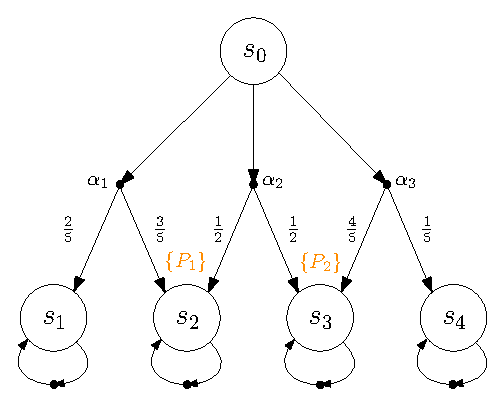
\includegraphics[width=0.8\linewidth]{resources/pareto-curve-MDP}
    \end{minipage}
    \begin{minipage}{0.5\linewidth}
      \centering
      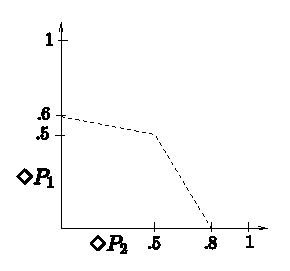
\includegraphics[width=0.7\linewidth]{resources/pareto-curve}
    \end{minipage}
    \captionsetup{justification=centering}
    \caption{MDP with $P_1 = \{s_2\}$, $P_2 = \{s_3\}$, two reachability events, $\Diamond P_1$ and $\Diamond P_2$, and the associated Pareto curve}
    \label{pareto-curve-example}
  \end{figure}
We are interested in the Pareto optimal vectors of the very simple following \MOSR{} problem:
$\mathcal{Q}:= ?\exists \sigma \; \bigwedge_{i=1}^2 \mathbb{P}^\sigma_{s_0}(\Diamond P_i) \geq 0$.
These Pareto optimal vectors describe the probabilities of strategies offering the \textit{optimal compromises} of reaching $P_1$ and $P_2$, i.e., the dominant probabilities of $\mathcal{Q}$.
We start from the state $s_0$ with enabled actions $\alpha_1$, $\alpha_2$, and $\alpha_3$.
By choosing $\alpha_1$, the system goes to $P_1$ with probability $0.6$ and $P_2$ with probability zero.
Then, if $\alpha_2$ is chosen, the system goes to $P_1$ and $P_2$ with probability $\frac{1}{2}$.
Finally, if $\alpha_3$ is chosen, the system goes to $P_1$ with probability zero and $P_2$ with probability $0.8$.
These three choices lead to the three Pareto optimal  vectors
$(0, 0.6)$, $(0.5, 0.5)$, and $(0.8, 0)$.
Indeed, none of these vectors can be dominated by
another vectors yielded from another strategies.
The three vertices of the Pareto curve of Figure \ref{pareto-curve-example} describe these three Pareto optimal vectors.
\end{example}


\subsection{Randomised strategies} \label{randomised-strategies}
Before detailing an algorithm to solve the \MOSR{} problem for a given state and given reachability properties in an MDP, we are going to interest us in type of strategies required for such a problem.
Indeed, let $\mathcal{M}$ be the MDP of Figure \ref{MDP-memory-1} and consider the \MOSR{} problem $\mathcal{Q}:= ?\exists \sigma \; \bigwedge_{i=1}^3 \mathbb{P}^\sigma_{s_0}(\Diamond T_i) = 1$.
It is clear that this problem requires memory.
Indeed, starting from $s_0$, as $T_1$ and $T_2$ have to be almost surely reached, the actions $\alpha_1$ and $\alpha_2$ have to be chosen by the strategy while $T_1$ or $T_2$ has not been reached yet.
When $T_1$ and $T_2$ have been reached, the strategy switches mode and chooses the action $\alpha_3$ in order to almost surely reach $T_3$.
\begin{figure}[h]
  \vspace{-.05\linewidth}
  \begin{minipage}{0.5\linewidth}
    \centering
    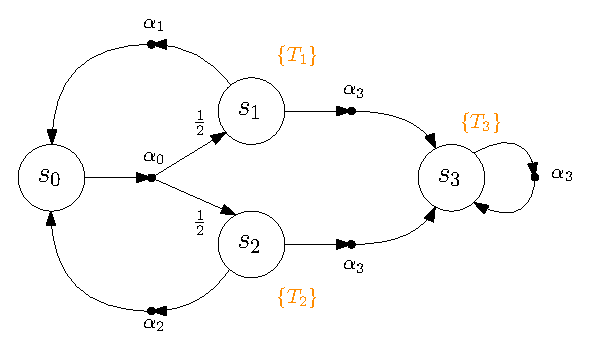
\includegraphics[width=0.9\linewidth]{resources/MDP-memory}
    \captionsetup{justification=centering}
    \captionof{figure}{MDP requiring memory to satisfy $\mathcal{Q}:= ?\exists \sigma \; \bigwedge_{i=1}^3 \mathbb{P}^\sigma_{s_0}(\Diamond T_i) = 1$}
    \label{MDP-memory-1}
  \end{minipage}
  \begin{minipage}{0.5\linewidth}
    \centering
    \vspace{.12\linewidth}
    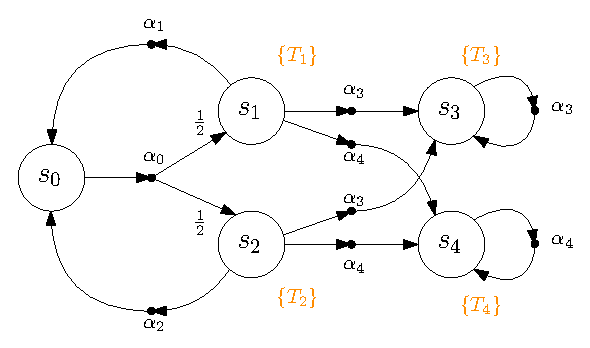
\includegraphics[width=0.9\linewidth]{resources/MDP-memory-2}
    \captionsetup{justification=centering}
    \captionof{figure}{MDP requiring both memory and randomisation to satisfy $\mathcal{Q}:= ?\exists \sigma \; \bigwedge_{i=1}^2 \mathbb{P}^\sigma_{s_0}(\Diamond T_i) = 1 \wedge \bigwedge_{i=3}^4 \mathbb{P}^\sigma_{s_0} (\Diamond T_i) \geq \frac{1}{2}$}
    \label{MDP-memory-2}
  \end{minipage}
\end{figure}
Actually, memory is not sufficient in some cases.
Indeed, assume that we slightly modify $\mathcal{M}$
(cf. Figure \ref{MDP-memory-2}) and consider the \MOSR{} problem
$\mathcal{Q}:= ?\exists \sigma \; \bigwedge_{i=1}^2 \mathbb{P}^\sigma_{s_0}(\Diamond T_i) = 1 \wedge \bigwedge_{i=3}^4 \mathbb{P}^\sigma_{s_0} (\Diamond T_i) \geq \frac{1}{2}$.
Again, a strategy $\sigma$ satisfying $\mathcal{Q}$ has to
choose actions $\alpha_1$ and $\alpha_2$ until that $T_1$ and $T_2$ are reached.
Then, the strategy switches mode in order to satisfy $\bigwedge_{i=3}^4 \mathbb{P}^\sigma_{s_0} (\Diamond T_i) \geq \frac{1}{2}$. Here, deterministically choosing between $\alpha_1$ and $\alpha_2$ is not sufficient: choosing $\alpha_3$ almost surely ensures to reach $T_3$ but implies reaching $T_4$ with probability zero,
and choosing $\alpha_4$ implies reaching $T_3$ with probability zero but almost surely ensures reaching $T_4$.
The optimal solution consists in choosing $\alpha_3$ and $\alpha_4$ with probability $\frac{1}{2}$.\\

Such strategies, choosing actions randomly, are \textit{randomised strategies}.
%For this \MOSR{} problem, both memory and randomisation are required, but we will see that we can solve some \MOSR{} problems only with randomisation.
In fact, getting back to Example \ref{pareto-example}, points on the dotted line of the Pareto curve of Figure \ref{pareto-curve-example} refer to strategies using randomisation.

\begin{definition}[\textbf{Randomised finite-memory strategies}]
  Let \sloppy $\mathcal{M}={(S, A, \Delta, w, AP, L)}$ be an MDP. A \textit{finite-memory randomised strategy} $\sigma = (Q, \sigma_{act}, \delta, \delta_0)$ is a \textit{stochastic Moore machine}, where
  \begin{itemize}
    %\item $Q, \delta, \delta_0$ are defined the same way as for pure finite-memory strategies, and
    \item $Q$ is a finite set of \textit{modes},
    \item $\sigma_{act}: Q \times S \rightarrow \mathcal{D}(A)$ is the \textit{stochastic next action function} giving, for each $s \in S$, a probability distribution on actions of $A(s)$ following a mode $q \in Q$ in which the machine is currently,
    \item $\delta: Q \times S \rightarrow \mathcal{D}(Q)$ is the \textit{stochastic transition function},
    \item $\delta_0: S \rightarrow Q$ is the \textit{initialisation function}, defined as for the pure strategy, giving the initial mode $q \in Q$, following a state $s \in S$ from which the machine is initialised.
  \end{itemize}
\end{definition}

According to this definition, the probability distribution defined on the successors of each state $s$ of a Markov chain induced by such a strategy additionally depends on the probability distribution defined on enabled actions of $s$ given by the stochastic next action function as well as the probability distribution defined on modes of the Moore Machine given by the stochastic transition function.

\begin{definition}[\textbf{Markov chain induced by a randomised finite-memory strategy}]
  Let $\mathcal{M}=(S, A, \Delta, w, AP, L)$ be an MDP and $\sigma=(Q, \sigma_{act}, \delta, \delta_0)$ be a randomised finite-memory strategy for $\mathcal{M}$.
  The product of $\mathcal{M}$ by $\sigma$ is given by
  \[
    \mathcal{M} \times \sigma = \mathcal{M}^\sigma = (S \times Q, \Delta^\sigma, AP, L^\sigma)
  \]
  where $\mathcal{M}^\sigma$ is the MC induced by the randomised finite-memory strategy $\sigma$ and where, for all states $s, s' \in S$, and for all modes $q, q' \in Q$,
  \begin{itemize}
    \item $\Delta^\sigma((s, q), (s', q')) =
    \delta(q, s)(q') \cdot \sum_{\alpha \in A(s)} \sigma_{act}(q, s)(\alpha) \cdot \Delta(s, \alpha, s')$
    \item $L^\sigma(s, q) = L(s)$.
  \end{itemize}
\end{definition}

\begin{remark}[\textit{Weight function in an MC induced by a randomised strategy}]
  We do not consider the weight function of any induced MC by a randomised strategy $\sigma$ in this context.
  Indeed, the weight of a transition depends on the action chosen by the strategy. Here, as actions are chosen randomly following a probability distribution defined on enabled actions of each state, this information is lost in the induced MC.
  It is however possible to define a weight function
  \[
    \overline{w}^\sigma: (S \times Q)^2 \rightarrow \mathbb{Q}_{>0}, \; ((s, q), (s', q')) \mapsto \delta(q, s)(q') \cdot \sum_{\alpha \in A(s)} \sigma_{act}(q, s)(\alpha) \cdot w(\alpha),
  \]
  referring to the expected weight of each transition in the induced MC, but this definition is irrelevant in this context.
\end{remark}

As for pure strategy, there exists a subset of randomised finite-memory strategies with only one mode for a given MDP.
These randomised strategies are \textit{memoryless}.

\begin{definition}[\textbf{Randomised memoryless strategy}]
  Let \sloppy$\mathcal{M}=(S, A, \Delta, w, AP, L)$ be an MDP. A randomised memoryless strategy $\sigma$ is a function
  $
    \sigma: S \rightarrow \mathcal{D}(A),
  $ giving, following a state $s \in S$, a probability distribution defined on the enabled action of $s$.
\end{definition}

\subsection{Multi-objective reachability with absorbing target \sloppy states} \label{MOSR-absorbing}

In this subsection, we present an efficient way to solve an \MOSR{} problem where the set of target states are only composed of absorbing states. More formally, let $\mathcal{M}=(S, A, \Delta, w, AP, L)$ be an MDP, and
$
  \mathcal{Q}_{s^*, r} := \,?\exists \sigma\; \bigwedge_{i=1}^r \mathbb{P}^\sigma_{s^*}(\Diamond T_i) \geq \alpha_i
$
be a \MOSR{} problem for $s^* \in S$, $r \in \mathbb{N}$, $(T_i)_{i \in \{1, \dots, r\}} \subseteq S^r$, and $\alpha \in ([0, 1] \cap \mathbb{Q})^r$.
We assume that for all $i \in \{ 1, \dots, r\}$ and for all targets $t \in T_i$, $t$ is absorbing, i.e., there exists an enabled action of $t$, $\alpha \in A(t)$, such that $\Delta(t, \alpha, t) = 1$.\\

In order to solve $\mathcal{Q}_{s^*, r}$, we need to do some preprocessing on $\mathcal{M}$, to ignore some useless and bad states.
Let $T = \bigcup_{i \in \{1, \dots, r\}} T_i$ and $S_{=0} = \{s \in S \; | \; \forall \sigma, \; \mathbb{P}_{s}^\sigma(\Diamond T) = 0\}$.
  Remind that this set can be computed efficiently in polynomial time in the size of $\mathcal{M}$ by checking if each state $s$ is connected to $T$ in the underlying graph of $\mathcal{M}$.
Let $\Delta_{>0} : S \times A \times S$ be the \textit{safe transition function} of $\mathcal{M}$, $s, s' \in S$, and $\alpha \in A(s)$, this function is defined as follows:
  \[
    \Delta_{>0}(s, \alpha, s') = \begin{cases}
      \Delta(s, \alpha, s') &\text{if } s \not \in S_{=0} \text{ and } s' \not\in S_{=0}, \\
      0 &\text{else}.
    \end{cases}
  \]
  %Let $A_{>0}(s) = \{ \alpha \in A(s) \; | \; \sum_{s' \in S} \Delta_{>0}(s, \alpha, s') > 0 \}$ be the set of \textit{safe enabled actions of the state $s \in S$}
  Let $s \in S$ and $\alpha \in A(s)$,
  by considering this transition function, we have \sloppy$\sum_{s' \in S} \Delta_{>0}(s, \alpha, s') \leq 1$, and furthermore,
      %$\Delta(s, \alpha, S_{=0}) =
      $\sum_{s' \in S_{=0}} \Delta(s, \alpha, s') =
      1 - \sum_{s' \in S} \Delta_{>0}(s, \alpha, s') $.
\begin{notation}[\textit{Cleaned-up MDP}]
  Defined as above, we say that the safe transition function $\Delta_{>0}$ \textit{clean-up} $\mathcal{M}$ for $T = \bigcup_{i \in \{1, \dots, r\}} T_i$.
\end{notation}

% \begin{figure}[h]
%   \centering
%   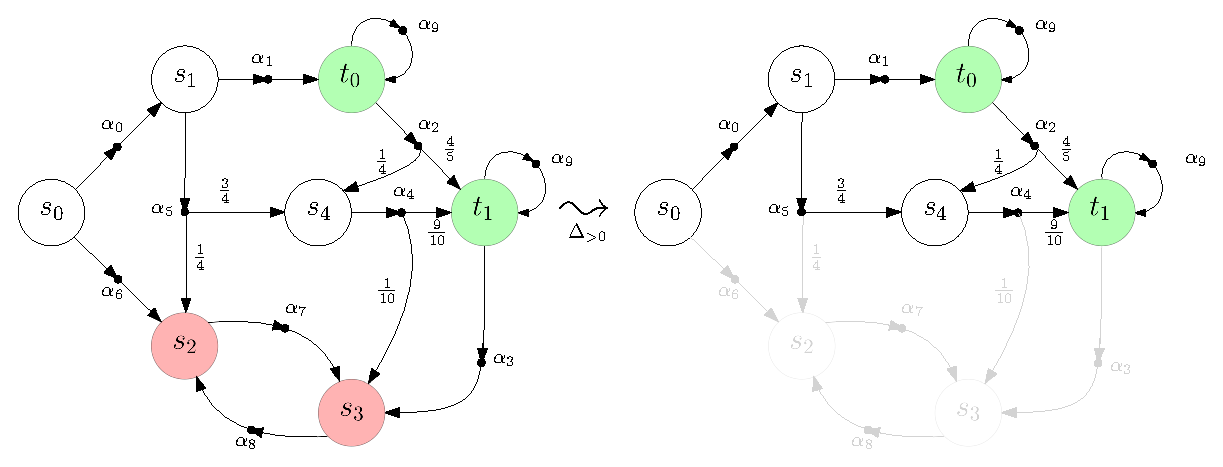
\includegraphics[width=0.9\linewidth]{resources/clean-up}
%   \caption{MDP cleaned-up with $\Delta_{>0}$ for $T = \{t_0, t_1\}$}
% \end{figure}


We are  going to define a \textit{multi-objective linear program} (MOLP, for short) to solve $\mathcal{Q}_{s^*, r}$.
An MOLP is defined the same way as a classical LP except that the optimisation consists in simultaneously maximising (or minimising) multiple objective functions.
A feasible solution of an MOLP is \textit{efficient} if it is a \textit{dominant solution}, i.e.,
where neither value of objective function can be optimised without degrading the value of another objective function.
Thus, the set of efficient solutions of an MOLP is a Pareto curve.\\

We assume that $\mathcal{M}$ is cleaned-up for $T = \bigcup_{i=1}^r T_i$ with $\Delta_{>0}$.
Let $(y_t)_{t \in T} \in \mathbb{Q}^r_{\geq 0}$, and $(y_{s, \alpha})_{s \in S \setminus T, \, \alpha \in A(s)} \in \mathbb{Q}_{\geq0}^r$. With these variables, we define the following MOLP:
\begin{figure}[h]
    \[\textbf{Objectives } i \in \{ 1, \dots, r\} \; : \;
   \max \sum_{t \in T_i} y_t\]
      subject to the following constraints:
    \begin{flalign}
       \mathds{1}(s) +
        \sum_{s' \in S} \sum_{\alpha' \in A(s')} \Delta_{>0}(s', \alpha', s) \cdot y_{s', \alpha'} &= \sum_{\alpha \in A(s)} y_{s, \alpha} && \forall s \in S \setminus T \label{eq1}\\
        \sum_{s' \in S \setminus T} \sum_{\alpha'\in A(s')} \Delta_{>0}(s', \alpha', t) \cdot y_{s', \alpha'} &= y_t && \forall t \in T \label{eq2} \\
        y_{s, \alpha} &\geq 0 && \forall s \in S \setminus T \text{ and } \alpha \in A(s) \notag \\
        y_t &\geq 0 && \forall t \in T \notag
    \end{flalign}
  \[\text{where } \mathds{1}(s) = \begin{cases}
    1 & \text{if } s=s^*,\\
    0 & \text{else}.
  \end{cases}\]
  \caption{MOLP for the \MOSR{} problem $\mathcal{Q}_{s^*, r}$}
  \label{molp}
\end{figure}

This MOLP is derived from the dual LP of the standard LP for single-objective reachability obtained from Bellman's equation for optimal reachability (cf. Theorem \ref{bellman1} and Appendix \ref{app-sr}).

\begin{theorem}%[\textbf{\textit{Multi-objective reachability with absorbing target states}}]
  [\textbf{\textit{Feasible solution and satisfying strategy}}]\label{feasible-strategy}
  Let $\mathcal{M}$ be an MDP with state space $S$,
% and $\mathcal{Q}_{s^*, r}$ be the \MOSR{} problem for the state $s^* \in S$ and the $r \in \mathbb{N}$ constraints described by multiples target sets $T_i \subseteq S$, for $i \in \{1, \dots, r\}$, where every target $t \in \bigcup_{i=1}^r T_i$ is an absorbing state, and probability thresholds $\alpha \in ([0, 1] \cap \mathbb{Q})^r$.
  Let $\mathcal{M}$ be an MDP with state space $S$,
  $s^* \in S$, multiples target sets $T_i \subseteq S$, for $i \in \{1, \dots, r\}$, where every target $t \in \bigcup_{i=1}^r T_i$ is an absorbing state, and a probability thresholds vector $\alpha \in ([0, 1] \cap \mathbb{Q})^r$.
  The two following propositions are equivalent:
  \begin{enumerate}[(a.)]
    \item There exists a randomised memoryless strategy $\sigma$ such that
    \[
      \bigwedge_{i=1}^r\mathbb{P}^\sigma_s(\Diamond T_i) \geq \alpha_i.
    \]
    \item There is a feasible solution $y'$ for the MOLP in Figure \ref{molp} such that
    \[
      \bigwedge_{i=1}^r \, \sum_{t \in T_i} y'_t \geq \alpha_i.
    \]
  \end{enumerate}
\end{theorem}
A proof of this theorem is provided in \cite{DBLP:journals/lmcs/EtessamiKVY08}.
Let $y'$ be a feasible solution of the MOLP in Figure \ref{molp}, we intuitively explain it as follows:
\begin{itemize}
  \item $y'_{s, \alpha}$, with $s \in S \setminus T, \, \alpha \in A(s)$, is the \textit{frequency} of the transition $s\xrightarrow{\alpha}$, i.e., the
  \textit{``expected number of time that %the underlying strategy of $y'$ chooses
  the action $\alpha$ is chosen
  to reach $T$
  when the system is in the state $s$"}.
  \item $\sum_{\alpha \in A(s)} y'_{s, \alpha}$, with $s \in S \setminus T$, is thus the \textit{visit frequency} of the state $s$, i.e., the \textit{``expected number of times that the state $s$ is visited to reach T"}
  %when the MDP is controlled by the underlying strategy of $y'$.
  (cf. constraint \ref{eq1}).
  \item $y'_t$, with $t \in T$, is the visit frequency of the state $t$ \textit{by states other than $t$}.
  Since $t$ is absorbing, this visit frequency can be translated into the probability of eventually reaching $T$ (cf. constraint \ref{eq2}).
\end{itemize}

Moreover, we can build a randomised strategy $\sigma$ from any feasible solution $y'$ of this MOLP.
Indeed, let $S_{freq>0} = \{ s \in S \setminus T \; | \;  \sum_{\alpha \in A(s)} y'_{s, \alpha} > 0 \} $ be the set of states with a nonzero visit frequency,
and $s \in S$, $\alpha \in A(s)$,
\begin{equation}
  \sigma(s)(\alpha) = \begin{dcases*}
    \frac{y'_{s, \alpha}}{\sum_{\alpha' \in A(s)} y'_{s, \alpha'}} & \text{if } $s \in S_{freq>0}$,\\[0.5em]
    \mu(s)(\alpha) & \text{else},
  \end{dcases*} \label{sigma_rand}
\end{equation}
where $\mu: S \rightarrow \mathcal{D}(A)$, and $\mu(s)$ is an arbitrary distribution on enabled actions of $s$.

\begin{corollary}[\textbf{\textit{Multi-objective reachability with absorbing target states}}]\label{mosr-absorbing-cor}  Let $\mathcal{M}$ be an MDP with state space $S$,
and $\mathcal{Q}_{s^*, r}$ be the \MOSR{} problem for the state $s^* \in S$ and the $r \in \mathbb{N}$ constraints described by target sets $T_i \subseteq S$, for $i \in \{1, \dots, r\}$, where every target $t \in \bigcup_{i=1}^r T_i$ is an absorbing state, and probability thresholds $\alpha \in ([0, 1] \cap \mathbb{Q})^r$.
\begin{enumerate}[(a.)]
  \item The \MOSR{} problem $\mathcal{Q}_{s^*, r}$ can be decided in polynomial time in the size of $\mathcal{M}$ and in the number of set of target states to reach (i.e., $r$), and if a strategy exists for this problem, we can build a randomised memoryless strategy that satisfies it. \label{mosr-cor1}
  %\item We can enumerate all Pareto optimal strategies satifying $\mathcal{Q}_{s^*, r}$ in \textit{output-polynomial} time. \label{mosr-cor3}
  \item For $\epsilon > 0$, we can compute an $\epsilon$-approximated Pareto curve $\mathpzc{P}(\epsilon)$ for the \MOSR{} problem $\mathcal{Q}_{s^*, r}$ in polynomial time in the size of $\mathcal{M}$ and $\frac{1}{\epsilon}$. \label{mosr-cor2}
\end{enumerate}
\end{corollary}

\begin{proof2}
  For \ref{mosr-cor1}, consider the MOLP in Figure \ref{molp} and add the constraint $\sum_{t \in T_i} y_t \geq \alpha_i$ for each $i \in \{1, \dots, r\}$. Then,
  forget the $r$ objective functions of this MOLP and consider the unique objective function $\max \sum_{i=1}^r\sum_{t \in T_i} y_t$.
  This yields a classical LP. If there exists an optimal solution to this LP, then we can
  build a randomised strategy from this solution (cf. Equation \ref{sigma_rand}).\\
  %\par The part. \ref{mosr-cor3} follows from Theorem \ref{feasible-strategy}: we see that we can build a strategy from a feasible solution of the MOLP in Figure \ref{molp}, and all efficient solution of this MOLP, i.e., all Pareto optimal solutions can be enumerated in \textit{output-polynomial time} (cf. \cite{Boros09generatingvertices}).
  %Ouput-polynomial time means that the problem is polynomial in the number of constraint of the MOLP, the number of objective, the size of their encoding representation, and the number of vertices of the Pareto curve of $\mathcal{Q}_{s^*, r}$.
  The part. \ref{mosr-cor2} directly follows from Theorem \ref{feasible-strategy} and the results of \cite{DBLP:conf/focs/PapadimitriouY00}. \flushright
\end{proof2}

\subsection{General multi-objective reachability}
We have presented a way to solve an \MOSR{} problem only involving sets of absorbing target states.
We present in this section a more general approach, without the absorbing restriction for target states.\\

Let $\mathcal{M}=(S, A, \Delta, w, AP, L)$ be an MDP, and
$
  \mathcal{Q}_{s^*, r} := \,?\exists \sigma\; \bigwedge_{i=1}^r \mathbb{P}^\sigma_{s^*}(\Diamond T_i) \geq \alpha_i
$
be a \MOSR{} problem for $s^* \in S$, $r \in \mathbb{N}$, $(T_i)_{i \in \{1, \dots, r\}} \subseteq S^r$, and $\alpha \in ([0, 1] \cap \mathbb{Q})^r$.
The technique we use to solve $\mathcal{Q}_{s^*, r}$ is inspired of which used in \cite{DBLP:journals/lmcs/EtessamiKVY08} to solve a multi-objective model-checking query for multiple \textit{$\omega$-regular properties} by doing the product of $\mathcal{M}$ with multiple \textit{Büchi automata} representing these properties.
Our technique requires to introduce the notion of
%\textit{transition table} and
\textit{end-components} of an MDP \cite{PMC}.

% \begin{definition}[\textbf{Deterministic transition table}]
%   A \textit{deterministic transition table} is a tuple $\tau = (\Sigma, Q, \delta)$, where $\Sigma$ is a finite alphabet, $Q$ is a finite set of states
%   and $\delta: S \times \Sigma \rightarrow S$ is a transition function.
% \end{definition}

\begin{definition}[\textbf{End component}]
  An \textit{end-component} (EC, for short) of an MDP $\mathcal{M} = (S, A, \Delta, w, AP, L)$ is an MDP $\mathcal{C}=(S^*, A^*, \Delta^*)$ such that
  \begin{itemize}
    \item $S^* \subseteq S$ and $S^* \neq \emptyset$,
    \item for all $s \in S^*$, $A^*(s) \subseteq A(s)$, $A^*(s) \neq \emptyset$, and
      for each $\alpha \in A^*(s)$,
      %$\Delta(s, \alpha, s') > 0 \implies s' \in S^*(s)$,
      $Succ(s, \alpha) \subseteq S^*$,
    \item $\Delta^* = \Delta |_{S^* \times A^*}$, and
    \item $\mathcal{C}$ is \textit{strongly connected}, i.e., there exists a path in $\mathcal{C}$ between any pair of states in $S'$.
  \end{itemize}
\end{definition}

\begin{definition}[\textbf{Maximal end-component}]
$\mathcal{C}=(S^*, A^*, \Delta^*)$ is a \textit{maximal end-component} of $\mathcal{M}$ if there is no end-component
$\mathcal{C}'=(S', A', \Delta')$ such that $(S^*, A^*) \neq (S', A')$ and $S^* \subseteq S'$ and $A^*(s) \subseteq A'(s)$ for all $s \in S^*$.
We let \MEC{}($\mathcal{M}$) denote the set of maximal ECs of $\mathcal{M}$, computable in polynomial time in the size of $\mathcal{M}$.
\end{definition}
The key properties of ECs that we are going to exploit in order to build a satisfying strategy for any \MOSR{} are the following.
\begin{lemma}[Recurrence property of end components]
  For end component $\mathcal{C}=(S^*, A^*, \Delta^*)$ of MDP $\mathcal{M}$, there exists a finite-memory strategy $\sigma$ for $\mathcal{M}$
  such that for any $s \in S^*$:
  \[
    \mathbb{P}^{\sigma}_s(\{ \pi \in Paths(s) \; | \; \pi \models \square S^* \; \wedge \; inf(\pi) = S^* \}) = 1.
  \]
\end{lemma}

\begin{theorem}[\textbf\textit{{Limiting behaviour of MDPs}}]\label{limit-ec-lemma}
  For each state $s$ of a finite MDP $\mathcal{M}$ and strategy $\sigma$ for $\mathcal{M}$:
  \[
  \mathbb{P}_s^\sigma(\{\pi \in Paths(s) \; | \; inf(\pi) \text{ is the state space of an EC
  of }\mathcal{M} \} ) = 1,
  \]
  i.e., whatever the strategy, each path starting in $s$ ends up in an EC of $\mathcal{M}$ almost surely.
\end{theorem}
Thus, any strategy of $\mathcal{M}$ almost surely ensures to reach an EC of $\mathcal{M}$, and once a state of this EC $\mathcal{C}$ is reached in $\mathcal{M}$,
there exists a strategy that almost surely enforces staying forever in $\mathcal{C}$ while visiting all of its states infinitely often.\\

% \begin{property}\label{ec-strategy}
% For each end-component $\mathcal{C}=(S^*, A^*, \Delta^*)$ of $\mathcal{M}$, once a state $S^*$ is reached in $\mathcal{M}$,
% there exists a strategy that almost surely enforce staying forever in $S^*$ while visiting all states in $S^*$ infinitely often.
% \end{property}
%
%Consider now the deterministic transition table $\tau_i = (S, \, \{0, 1\}, \, \delta_i)$ for each $i \in \{1, \dots, r\}$, where the transition function $\delta_i: \{0, 1\} \times S \rightarrow \{0,1\}$ is defined as follows:

For each reachability property $i \in \{1, \dots, r\}$, we define a \textit{reachability transition function} $\delta_i: \{0, 1\} \times S \rightarrow \{0,1\}$ as follows:
\[
  \delta_i(q, s) = \begin{cases}
    1 & \text{if } q=1 \text{ or } s \in T_i \\
    0 & \text{else.}
  \end{cases}
\]
% The behaviour of this transition function is depicted in Figure \ref{transition-table}.
% \begin{figure}[h]
%   \centering
%   \captionsetup{justification=centering}
%   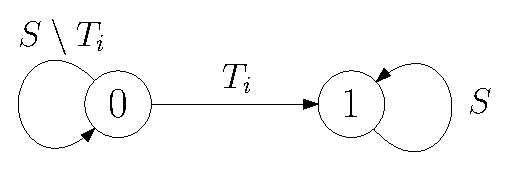
\includegraphics[width=0.37\linewidth]{resources/transition-table}
%   \caption{Behaviour of the reachability transition function $\delta_i$ for the reachability to $T_i$}
%   \label{transition-table}
% \end{figure}
% Its behaviour is quite simple and describes the reachability to the subset of target states $T_i$ in $\mathcal{M}$: we begin with a boolean variable $q$, and we incrementally update the value of this variable with the transition function $\delta_i$.
% If this boolean value is initialised with $1$, then the transition function will always return the value $1$, and the value of the variable always equals $1$,
% regardless of the value of the state read by the $\delta_i$.
% If $q$ equals $0$, then, its next value depends on the state read. If the state read is in $T_i$, then the variable $q$ is updated with $1$, else the next value of $q$ stills $0$.
% If we initialise $q$ with $0$ and apply the transition function $\delta_i$ along a path $\pi = s_0 \xrightarrow{\alpha_1} s_1 \xrightarrow{\alpha_2} s_2 \xrightarrow{\alpha_3} \dots \in Paths(s^*)$,
% we incrementally update the value of this variable $q$ reading the state $s_{k+1}$ for each transition $s_k \xrightarrow{\alpha_{k+1}}s_{k+1}$ of $\pi$.
% Following this way, when a state of $T_i$ is reached along $\pi$, the boolean variable $q$ is $1$.
% Contrariwise, if $T_i$ is never reached along this path, the variable $q$ is always $0$. \\
In order to solve $\mathcal{Q}_{s^*, r}$, we build a new MDP $\mathcal{M}'=(S', A', \Delta')$ with each of these reachability transition functions, defined as follows:
\begin{itemize}
  \item $S' \subseteq (S\, \cup\, \{s_0\}) \times \{0, 1\}^r$ is composed of states $(s, q_1, \dots, q_r)$ such that $s \in S$, $(q_1, \dots, q_i) \in \{0, 1\}^r$, intuitively recording through the boolean variable $q_i$ if $T_i$ has been reached along a path starting from $s^*$, for each $i \in \{1, \dots, r\}$.
  We additionally add a dummy state $(s_0, 0, \dots,0)$ in $S'$.
  \item $A' = A \cup \{\alpha_0\}$ and $A'(s, q_1, \dots, q_r) = A(s)$ for all $(s, q_1, \dots, q_r) \in S'$, and $A'(s_0, 0, \dots, 0) = \{\alpha_0\}$.
  \item $\Delta'$ is a probability transition function, defined as follows: let $x=(s, q_1, \dots, q_r) \in S'$, $x' = (s', q_1', \dots, q'_r) \in S'$, and $\alpha \in A'(x)$,
  \[
  \Delta(x, \alpha, x') = \begin{dcases*}
    1 & if $s = s_0$, $s'=s^*$, and $\forall i \in \{1, \dots, q\}$, $\delta_i(q_i, s) = q'_i$, \\
    \Delta(s, \alpha, s') & if $s, s'\in S$ and  $\forall i \in \{1, \dots, q\}$, $\delta_i(q_i, s) = q'_i$,\\
    0 & otherwise.
  \end{dcases*}
  \]
  This probability transition function suggests the additional dummy transition $(s_0, 0, \dots, 0) \xrightarrow{\alpha_0} (s^*,\, \delta_1(0, s^*), \dots,\, \delta_r(0, s^*))$, with probability one.
  If this transition is not added, $s^*$ is never read by the reachability transition function $\delta_i$, which could be a problem if $s^* \in T_i$ for some $i \in \{1, \dots, r\}$.
\end{itemize}
Furthermore, as we consider paths of $\mathcal{M}$ starting from $s^*$, we limit the state space $S'$ with the states reachable from $(s_0, 0, \dots, 0)$.

\begin{definition}[\textbf{Favoured reachability property}]
  Let $\mathcal{C}=(S^*, A^*, \Delta^*)$ be an EC of $\mathcal{M}$, we say that $\mathcal{C}$ favours a set of reachability property $R \subseteq \{1, \dots, r\}$ if and only if
    for all $(s, q_1, \dots, q_r) \in S^*$ and for all $i \in R$,  $q_i = 1$.
\end{definition}

\begin{lemma}[Favoured reachability and property of end-components] \label{lemma-favour}  Let $\mathcal{C} = (S^*, A^*, \Delta^*)$ be an EC of $\mathcal{M}'$, and $(s, q_1, \dots, q_r) \in S^*$ be any state of $\mathcal{C}$, then $\mathcal{C}$ favours all the subsets of $R = \{ i \in \{1, \dots, r\} \; | \; q_i = 1\}$ ($R$ included).
  Moreover, for all $(s', q'_1, \dots, q'_r) \in S^*$, $q'_i = 0$ for $i \in \{1, \dots, r\} \setminus R$.
\end{lemma}
\begin{proof2}
Let $(s, q_1, \dots, q_r)\in S^*$ be any state of $\mathcal{C}$,  $R = \{ i \in \{1, \dots, r\} \; | \; q_i = 1\}$, $S_R = \{ (s, q_1, \dots, q_r) \in S' \; | \; \forall i \in R, \, q_i = 1 \}$ and $s_R = (s, q_1, \dots, q_r) \in S_R$.
Actually, by definition of $\Delta'$ and $\delta_i$ for all $i \in \{1, \dots, r\}$, for all $\alpha \in A(s_R)$, $Succ(s_R, \alpha) \subseteq S_R$.
Thus, as any EC is strongly connected,
if there exists a state $(s, q_1, \dots, q_r) \in S^*$ such that $q_i = 1$ for all $i \in R$, then $S^* \subseteq S_R$. {\color{umons-red}(1.)} \\
Moreover, let $i \in \{1, \dots, r \} \setminus R$, and assume we have a state $u = (s, q_1, \dots, q_r) \in S^*$ with $q_i = 0$ such that there exists an $\alpha$-successor $(s', q'_1, \dots, q'_r) \in Succ(u, \alpha)$ for $\alpha \in A^*(s)$, with $q'_i = 1$, then, by {\color{umons-red}(1.)}, $q_i = 1$, that leads a contradiction.
\end{proof2}

\begin{lemma}[Multiple reachability in $\mathcal{M}'$] \label{MOSR-lemme}
Defined as above, $\mathcal{M}'$ has the following properties: for each $R \in 2^{\{1, \dots, q\}}$, there is a subset of target states $T_R \subseteq S'$ that satisfies the following conditions:
\begin{enumerate}[(1.)]
  \item If a path starting from $(s_0, 0, \dots, 0)$ visit a state in $T_R$ at some point, then
  % all strategy we can apply from that point on ensure that all the sets $T_i$, $i \in R$, are almost surely reached (i.e., with conditional probability one, conditioned on the visit of $T_R$).
  all the sets $T_i$, $i \in R$, have been reached along this path.
  \label{Mprime1}
  \item For every strategy, the set of paths reaching all sets of target states $T_i$, $i \in R$, and never visit some state of $T_R$ has probability zero. \label{Mprime2}
\end{enumerate}
All the sets $T_R$ can be computed simultaneously
in polynomial time in the size of $\mathcal{M}'$.
\end{lemma}

\begin{proof2}
  %We compute the set $\MEC{}(\mathcal{M}')$ (in polynomial time in the size of $\mathcal{M}'$), and we look for all the maximal ECs $\mathcal{C}=(S^*, A^*, \Delta^*)$ in this set such that each state $(s, q_1, \dots, q_r) \in S^*$ agrees with $q_i = 1$ for all $i \in R$. The union of the state space of each of these ECs forms the set $T_R$.
  Let $R \in 2^{\{1, \dots, r\}}$.
  We are going to look at all maximal end-components of $\mathcal{M}'$ favouring $R$ in order to define $T_R$.
  More formally, let $S_R = \{ (s, q_1, \dots, q_r) \in S' \; | \; \forall i \in R, \, q_i = 1 \}$ and $S^{\mathcal{C}}_R = \{ S^* \subseteq S_R \; | \; \exists \mathcal{C} \in \MEC(\mathcal{M'}) \text{ with state space } S^* \}$,
  \[
    T_R = \bigcup_{S^* \in S_R^\mathcal{C}} S^*.
  \]
  As $\MEC(\mathcal{M'})$ can be computed in polynomial time in the size of $\mathcal{M'}$, we can compute at a time all sets $T_R$ for all $R \in \{1, \dots, r\}$.
  \\
  %\ref{Mprime1}
  %We have that if a state $s_R = (s, q_1, \dots, q_r) \in T_R$ agrees with $q_i = 1$ for all $i \in R$, then $s_R \in T_R$, and for all $\alpha \in A'(s_R)$, $Succ(s_R, \alpha) \subseteq  T_R$.
  %Indeed,
  By definition of $\Delta'$ and by definition of $\delta_i$, for each $i \in R$, if a state $t=(s, q_1, \dots, q_r) \in S'$ is visited at some point with $s \in T_i$, then the boolean value $q_i$ is updated with $1$ (this is actually the only condition needed for $q_i$ to go from $0$ to $1$) and remains $1$ forever, i.e., for all
  $\pi=s_0 \xrightarrow{\alpha_1} s_1 \xrightarrow{\alpha_2}\dots \in Paths(t)$, for all $k \in \mathbb{N}$,
  we have $s_k = (s', q'_1, \dots, q'_r)$, with $q'_i =1$. {\color{umons-red}(*)} \\
  Thus, assume that a state in $T_R$ is reached along a path $\pi=s_0 \xrightarrow{\alpha_1} s_1 \xrightarrow{\alpha_2}\dots \in Paths((s_0, 0, \dots, 0))$, i.e., assume there exists an index $k \in \mathbb{N}$ such that $s_k = (s, q_1, \dots, q_r) \in T_R$. We have by definition of $T_R$ that $q_i = 1$ for all $i \in R$.
  Then, as the path starts from $(s_0, 0, \dots, 0)$ and by {\color{umons-red}(*)}, there exists for all $i \in R$ an index $k' \leq k$ such that $s_{k'} = (s', q'_1, \dots, q'_r)$
  with $s' \in T_i$. We have shown \ref{Mprime1}.\\
  Now, let $\sigma$ be a strategy for $\mathcal{M}'$ and $\pi %= s_0 \xrightarrow{\alpha_1}s_1 \xrightarrow{\alpha_2} \dots
  \in Paths^\sigma((s_0, 0, \dots, 0))$.
  Assume that all the sets of target states $T_i$ have been reached for $i \in R$ along $\pi$.
  By Lemma \ref{limit-ec-lemma}, this path ends up in an EC almost surely. By {\color{umons-red}(*)}, we necessarily have that this EC favours $R$, as all the target states $T_i$ have been reached. Thus, as $T_R$ is the union of the state space of each EC favouring $R$,
  \[
    \mathbb{P}^\sigma_{(s_0, 0, \dots, 0)}(\{ \pi \in Paths((s_0, 0, \dots, 0)) \; | \; inf(\pi) \subseteq T_R \}) = 1,
  \]
  which directly implies
  \[
    \mathbb{P}^\sigma_{(s_0, 0, \dots, 0)}(\{ \pi \in Paths((s_0, 0, \dots, 0)) \; | \; inf(\pi) \cap T_R = \emptyset \}) = 0.
  \]
  We are done with \ref{Mprime2}. That concludes the proof.
  \end{proof2}
  $ $\\

The Lemma \ref{lemma-favour} and the Lemma \ref{MOSR-lemme} allow us to define an algorithm ensuring to solve any \MOSR{} problem (cf. Algorithm \ref{mosr-algo}). The key idea behind this algorithm is that we add a new absorbing state $s_R$ in $\mathcal{M'}$ for each subset of constraints $R \subseteq \{1, \dots, r\}$.
Then, for each state $t \in S'$, and for each maximal subset $R$ such that $t \in T_R$, we add a new transition from $t$ to $s_R$.
By considering the new sets of target states $F_i = \{ s_R \; | \; i \in R\}$, for $i \in \{1, \dots, r\}$,
we solve the \MOSR{} problem for these sets of absorbing target states and the thresholds $\alpha \in [0,1]^r$ as described in Subsection \ref{MOSR-absorbing}.

\begin{algorithm}[h!]
\caption{Multi-objective reachability}\label{mosr-algo}
\begin{algorithmic}[1]
\REQUIRE{
  $\mathcal{M}=(S, A, \Delta, AP, L)$, a finite MDP, and $\mathcal{Q}_{s^*, r}$, a \MOSR{} problem.
}
\ENSURE{
  A strategy satisfying $\mathcal{Q}_{s^*, r}$ if it is possible to answer $True$ to $\mathcal{Q}_{s^*, r}$, $False$ else.
}
\STATE {\sffamily build} $\mathcal{M}'=(S', A', \Delta')$ with $\delta_i$, ${i \in \{1, \dots r\}}$
\FOR{$R \in 2^{\{1, \dots, r\}}$}
  \STATE $T_R \leftarrow \emptyset$
\ENDFOR
\FOR{$\mathcal{C}=(S^*, A^*, \Delta^*) \in \MEC(\mathcal{M}')$}
  \STATE {\sffamily let} $(s, q_1, \dots, q_r)$ be an arbitrary state of $S^*$
  \COMMENT{cf. Lemma \ref{lemma-favour}}
  \STATE $R^* \leftarrow \{ i \in \{1, \dots, r\} \; | \; q_i = 1 \}$
  \COMMENT{maximal subset of $\{1, \dots, r\}$ favoured by $\mathcal{C}$}
  \FOR{$R \subseteq R^*$}
    \STATE $T_R \leftarrow T_R \cup S^*$
  \ENDFOR
\ENDFOR
\FOR{$R \in 2^{\{1, \dots, r\}} \setminus \emptyset$}
  %\STATE $T_R \leftarrow \{ (s, q_1, \dots, q_r) \in S' \; | \; \forall i \in R,\, q_i=1 \}$
  %\STATE $T_R \leftarrow \{ (s, q_1, \dots, q_r) \in S' \; | \; \forall i \in R,\, q_i=1 \}$
  \STATE $S' \leftarrow S' \cup \{s_R\}$
  \STATE $A' \leftarrow A' \cup \{\alpha_R\} ; \; A'(s_R) \leftarrow \{\alpha_R\}$
  \STATE {\sffamily add} the transition $s_R \xrightarrow{\alpha_R}s_R$ in $\mathcal{M'}$ with $\Delta'(s_R, \alpha_R, s_R) = 1$
  %\COMMENT{we add a new absorbing state $s_R$ for all $R$}
\ENDFOR
% \FOR{$\mathcal{C} = (S^*, A^*, \Delta^*) \in \MEC(\mathcal{M'})$}
%   \STATE {\sffamily let} $(s, q_1, \dots, q_r)$ be an arbitrary state of $S^*$
%   \STATE $R \leftarrow \{ i \in \{1, \dots, r\} \; | \; q_i = 1 \}$
%   \COMMENT{maximal subset of $\{1, \dots, r\}$ favoured by $\mathcal{C}$}
%   %\FOR{$R \in R'$}
%   \STATE $T_R \leftarrow T_R \cup S^*$
%   %\ENDFOR
\FOR{$t \in \bigcup_{\mathcal{C}=(S^*, A^*, \Delta^*) \in \MEC(\mathcal{M'})} S^*$}
  \STATE {\sffamily let} $R \in 2^{\{1, \dots, r\}}$ be the maximal subset  of $\{1, \dots, r\}$ such that $t \in T_R$ \label{line-max-subset}
      \STATE $A'(t) \leftarrow A'(t) \cup \{\alpha_R\}$
      \STATE {\sffamily add} the transition $t \xrightarrow{\alpha_R}s_R$ in $\mathcal{M}'$ with $\Delta'(t, \alpha_R, s_R) = 1$
\ENDFOR
\FORALL{$i\leftarrow 1$ to $r$}
  \STATE $F_i \leftarrow \{ s_R \; | \; i \in R \}$
\ENDFOR
\STATE {\sffamily let} $\mathcal{Q}_{(s_0, 0 \dots, 0),\, r}$ be the \MOSR{} problem for the set of \textbf{absorbing target states} $F_i$ and cost thresholds $\alpha_i$ for $i \in \{1, \dots, r\}$ in $\mathcal{M}'$, from the state $(s_0, 0, \dots, 0)$.
\STATE {\sffamily solve} $\mathcal{Q}_{(s_0, 0, \dots, 0),\, r}$ \COMMENT{cf. Corollary \ref{mosr-absorbing-cor}}
\IF{there exists a strategy $\sigma'$ for $\mathcal{Q}_{(s_0,, 0, \dots, 0),\, r}$}
  \STATE {\sffamily build} $\sigma'$ for $\mathcal{M}'$
  \COMMENT{cf. Equation \ref{sigma_rand}}
  \RETURN $\sigma'$
\ELSE
  \RETURN $False$
\ENDIF
% \FOR{$(s, q_1, \dots, q_r) \in S'$}
%   \STATE $R' \leftarrow \emptyset$
%   \FOR{$i \leftarrow 1$ to $r$}
%     \IF{$q_i$}
%       \STATE$R' \leftarrow R' \cup \{i\}$
%     \ENDIF
%   \ENDFOR
%   \STATE $T_{R'} \leftarrow T_{R'} \cup \{ (s, q_1, \dots, q_r) \}$
% \ENDFOR
\end{algorithmic}
\end{algorithm}

\begin{lemma}[Recover a strategy for $\mathcal{M}$ from $\mathcal{M}'$]
  The sets of achievable points $U_{\mathcal{Q}_{s^*, r}} = U_{\mathcal{Q}_{(s_0,0, \dots, 0),\, r}}$. Moreover, from a randomised memoryless strategy $\sigma'$ that satisfies $\mathcal{Q}_{(s_0, 0, \dots, 0), \, r}$ in $\mathcal{M}'$, we can recover a randomised finite-memory strategy $\sigma$ that satisfies $\mathcal{Q}_{s^*, r}$ in $\mathcal{M}$.
\end{lemma}

\begin{proof2}
  Let $\sigma'$ be a strategy for the MDP $\mathcal{M}'$ of Algorithm \ref{mosr-algo}.
  Assume that $\mathcal{Q}_{(s_0, 0, \dots, 0),\, r}$ is satisfied by $\sigma'$. Thus, we have $\bigwedge_{i=1}^r\mathbb{P}_{(s_0, 0, \dots, 0)}^{\sigma'}(\Diamond F_i) \geq \alpha_i$.
  The strategy $\sigma$ for $\mathcal{M}$ skips the first choice of $\sigma'$ (necessarily being $\alpha_0$), and follows then the choices of $\sigma'$ in $\mathcal{M}$ from $s^*$ until just before it transitions to a state $s_R$, at which point it must be in a state $t \in T_R$, with $R$ being a maximal set of $\{ R' \subseteq \{1, \dots, r\} \; | \; t \in T_{R'} \}$, and at
  that point our strategy $\sigma$ switches to the strategy allowing to almost surely visiting all states of $T_R$. That guarantees that $\mathbb{P}_{s^*}^\sigma(\Diamond T_i) \geq \mathbb{P}_{(s_0, 0, \dots, 0)}^{\sigma'}(\Diamond F_i) \geq \alpha_i$, for all $i \in \{1, \dots, r\}$.
\end{proof2}

\begin{theorem}[\textbf{\textit{Solving the \MOSR{} problem}}] \label{theorem-mosr-final}
  Given an MDP $\mathcal{M}$ with state space $S$, we can solve the \MOSR{} problem for the state $s \in S$, the $r \in \mathbb{N}$ reachability properties described by the set of target states $T_i \subseteq S$ and the probability threshold $\alpha_i$ for each $i \in \{1, \dots, r\}$ in polynomial time in the size of $\mathcal{M}'$, i.e., in
  polynomial time in the size of $\mathcal{M}$ but in exponential time in the number of reachability properties $r$, and if so we can build a randomised exponential-memory strategy satisfying the problem.
  Moreover, we can build an $\epsilon$-approximated Pareto curve $\mathpzc{P}(\epsilon)$ in time polynomial in $\mathcal{M}$ and in $\frac{1}{\epsilon}$, but exponential time in the number of reachability properties $r$.
\end{theorem}

\begin{example}[\textit{Applying Algorithm \ref{mosr-algo} on a simple MDP}]
Let $\mathcal{M}$ be the MDP of Figure \ref{molp-mdp}. We are interested to know if there exists a strategy $\sigma$ such that
\[
  \underbrace{\mathbb{P}_{s_0}^{\sigma}(\Diamond \{s_1\}) \geq 0.8}_{\text{reachability property $1$}} \; \wedge \; \underbrace{\mathbb{P}_{s_0}^\sigma (\Diamond \{s_2\}) = 1}_{\text{reachability property $2$}}.
\]
\begin{figure}[h!]
  \centering
  \captionsetup{justification=centering}
  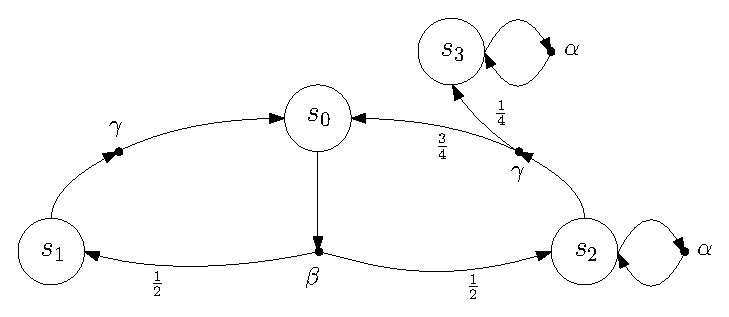
\includegraphics[width=0.7\linewidth]{resources/MOLP-simple-mdp}
  \caption{Simple MDP $\mathcal{M}$ with state space $S = \{s_0, s_1, s_2, s_3\}$ and action space $A = \{\alpha, \beta, \gamma\}$}
  \label{molp-mdp}
\end{figure}
\begin{figure}[h!]
  \centering
  \captionsetup{justification=centering}
  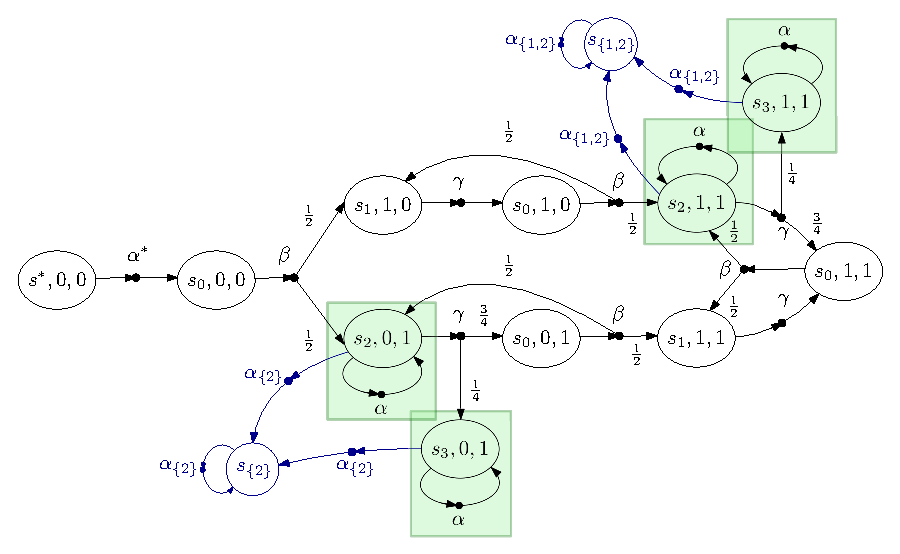
\includegraphics[width=0.9\linewidth]{resources/MOLP-product}
  \caption{MDP $\mathcal{M}'$ resulting of the modification of $\mathcal{M}$ in Algorithm \ref{mosr-algo}}
  \label{molp-mdp2}
\end{figure}
As $s_1$ is not absorbing, we cannot use the technique described in Subsection \ref{MOSR-absorbing} to solve this \MOSR{} problem.
We apply Algorithm \ref{mosr-algo} and build the associated MDP $\mathcal{M}'$ to solve the problem (cf. Figure \ref{molp-mdp2}).
The MECs of $\mathcal{M}'$ are the sub-MDPs highlighted in green, and the state spaces of these MECs form the sets $T_R$, with $R \in 2^{\{1, 2\}}$, following the reachability properties $i \in R$ that each MEC favours.
Here, the MEC containing the unique state $(s_2, 0, 1)$ and the one containing $(s_3, 0, 1)$ favour the second reachability property and thus are in $T_{\{2\}}$.
Then, the MEC containing the state $(s_2, 1, 1)$ and the one containing $(s_3, 1, 1)$ favour the properties $1$ and $2$ and thus are is $T_{\{1\}}$, $T_{\{2\}}$, and $T_{\{1, 2\}}$.
We then add the new absorbing target states $s_R$, for each subset of properties $R \subseteq \{1, \dots, r\}$, and we add a new transition from all states of each MEC $\mathcal{C}$ to $s_R$ such that $R$ is the maximal subset of properties favoured by $\mathcal{C}$ (in Figure \ref{molp-mdp2}, we ignore the target states $s_R$ unconnected to MECs of $\mathcal{M}'$).
We finally define the new set of absorbing target states $F_i = \{s_R \; | \; i \in R\}$ for $i \in \{1, \dots, r\}$, i.e., $F_1 = \{s_{\{1, 2\}}\}$ and $F_2 = \{s_{\{2\}}, \, s_{\{1, 2\}}\}$.
It remains to decide if there exists a strategy $\sigma'$ satisfying
\[
  \mathbb{P}^{\sigma'}_{(s^*, 0, 0)}(\Diamond F_1) \geq 0.8 \; \wedge \; \mathbb{P}_{(s^*, 0, 0)}^{\sigma'}(\Diamond F_2) = 1.
\]
\end{example}

\section{Percentile queries in multi-dimensional Markov decision processes}
In this section, we define some strategies allowing to deal with multiple \textit{percentile queries} in \textit{multi-dimensional Markov decision processes} \cite{DBLP:journals/fmsd/RandourRS17}.
A multi-dimensional MDP is an MDP where the weight of each action has multiple dimensions.
Remind the \SSPP{} problem in Section \ref{vssp} from Chapter \ref{preliminaries}, consisting in deciding the existence of a strategy satisfying one single percentile query.
We are now interested in defining a strategy solving \textit{simultaneously} multiple \SSPP{} problems on different weight dimensions and for different set of target states.

\begin{definition}[\textbf{Multi-dimensional Markov decision process}]
  A $d$-dimensional MDP is a tuple $\mathcal{M}=(S, A, \Delta, w, AP, L)$ where
  \begin{itemize}
    \item $S, A, \Delta, AP, L$ are defined as for classical MDPs, and
    \item $w$ is a $d$-dimension weight function $w: A \rightarrow \mathbb{N}_0^d$.
    For $k \in \{1, \dots, d\}$, we denote $w_k:A\rightarrow\mathbb{N}_0$ the projection of $w$ on the $k^\text{th}$ dimension, i.e., the function mapping each action $\alpha$ to the $k^\text{th}$ element of the vector $w(\alpha)$.
  \end{itemize}
\end{definition}

\begin{example}[\textit{Multi-dimensional MDP for the wireless sensor network}]
  We update the MDP presented in Example \ref{spg-example} in order to fill in the details left open in the situation described in Example \ref{main-example}.
  \begin{figure}[h]
    \centering
    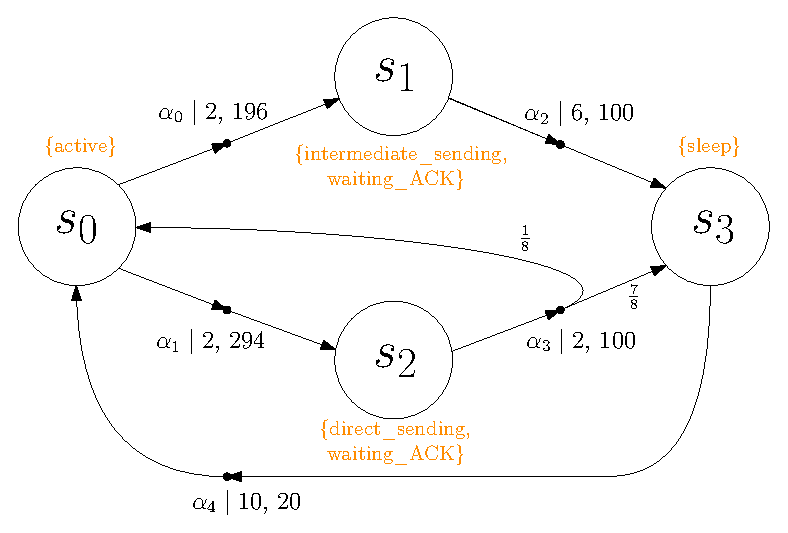
\includegraphics[width=0.6\linewidth]{resources/mdmdp2}
    \captionsetup{justification=centering}
    \caption{Multi-dimensional MDP modelling the situation of Example \ref{main-example}}
    \label{multi-mdp}
  \end{figure}
  We modify the weight function in order to support the energy cost of each action. This modification yields the MDP of Figure \ref{multi-mdp}.
  We assume here that waiting an ACK from a node uses $100$ \textit{mili Joules} ($mJ$), sending a message to $n_1$ uses $196$ $mJ$, sending a message to $n_2$ uses $294$ $mJ$, and staying in the \textit{sleep} state during $10$ $ms$ uses $20$ $mJ$.
\end{example}

\begin{remark}[\textit{Truncated sum in a multi-dimensional MDP}]
  The truncated sum function $\TS$ must be slightly modified in order to handle multidimensional MDPs.
  Indeed, let $\mathcal{M}$ be a $d$-dimensional MDP with state space $S$ and weight function $w$.
  We denote by $\TS^T_{k}$ the truncated sum up to $T$ on the $k^\text{th}$ dimension, with $k \in \{1, \dots, d\}$.
  More formally, let $\pi = s_0 \xrightarrow{\alpha_1} s_1 \xrightarrow{\alpha_2} s_2 \xrightarrow{\alpha_3} \dots \in Paths(s)$ be a path of $\mathcal{M}$ starting from $s \in S$,
  \[
  \TS^T_k(\pi) = \begin{cases}
    \sum_{i=1}^{n} w_k(\alpha_i) & \text{if } \forall i \in \{0, \dots, n-1\}, \, s_{i} \not\in T \, \wedge \, s_n \in T, \\
    + \infty & \text{else}.
  \end{cases}
  \]
  Furthermore, let $\sigma$ be a strategy for $\mathcal{M}$, we can define the event $\Diamond_{k: \, \leq \ell} \, T$ on $\sigma$-paths  starting from $s \in S$ as follows:
  \[
    \Diamond_{k:\,\leq \ell}\,T=\{\pi \in Paths^\sigma(s) \; | \; \TS^T_k(\pi) \leq \ell \}.
  \]
\end{remark}

\begin{definition}[\textbf{\SSPPQ{} problem}]
  Let $\mathcal{M}=(S, A, \Delta, w, AP, L)$ be a $d$-dimensional MDP, $s \in S$, and $q \in \mathbb{N}$ percentile constraints. These percentile constraints are described by a set of target states $T_i \subseteq S$, the dimensions $k_i \in \{1, \dots, d\}$, the cost thresholds $\ell_i \in \mathbb{N}$, and the probability thresholds $\alpha_i \in [0, 1] \cap \mathbb{Q}$, for each $i \in \{1, \dots, q\}$.
  The \textit{stochastic shortest path percentile queries} problem (\SSPPQ{}, for short) consists in deciding if there exists a strategy $\sigma$ such that
  \[
    \bigwedge_{i=1}^r \mathbb{P}^\sigma_s(\Diamond_{k_i:\, \leq \ell_i}\, T_i) \geq \alpha_i.
  \]
\end{definition}

\begin{example}[\textit{\SSPPQ{} problem in the wireless sensor network}] \label{SSPQ-example1}
  Let $\mathcal{M}$ be the MDP of Figure \ref{multi-mdp}, modelling the situation described in Example \ref{main-example} for the node $n_0$.
  We are interested to satisfy multiple percentile queries in $\mathcal{M}$, from the state $s_0$ (i.e., the \textit{active} state of the sensor $n_0$).
  Firstly, we want to ensure with a probability of $80 \%$ that the message will be sent to the sensor $n_2$ and acknowledged within $4 \; ms$ (cf. query $\mathcal{Q}_1$). Secondly, we want to ensure with a probability of $90 \%$ that the message will be sent to the sensor $n_2$ and acknowledged with an energy cost inferior or equal than $700 \; mJ$ (cf. query $\mathcal{Q}_2$).
  \begin{align*}
    &\bigcdot\;\mathcal{Q}_1 := \,  ?\exists \sigma \;\; \mathbb{P}^{\sigma}_{s_0}(\Diamond_{1: \, \leq 4} \, \{s_3\}) \geq 0.8 \\
    &\bigcdot\;\mathcal{Q}_2 := \, ? \exists \sigma \;\; \mathbb{P}_{s_0}^{\sigma}(\Diamond_{2: \, \leq 700} \, \{s_3\}) \geq 0.9
  \end{align*}
  Let $\sigma_1$ and $\sigma_2$ be two pure memoryless strategies for $\mathcal{M}$ such that
  \begin{itemize}
    \item $\sigma_1$ corresponds to the strategy always trying a direct sending to $n_2$, and
    \item $\sigma_2$ corresponds to the strategy sending the message via $n_1$.
  \end{itemize}
  The strategy $\sigma_1$ satisfies $\mathcal{Q}_1$ but does not satisfies $\mathcal{Q}_2$.
  Indeed, this strategy yields %on $Paths^{\sigma_1}(s_0)$
  the events
  \[\Diamond_{1:\, \leq 4}\, \{s_3\} = \Diamond_{2:\, \leq 700}\, \{s_3\} = \{ \pi \in Paths^{\sigma_1}(s_0) \; | \; s_0 %\xrightarrow{\alpha_1}
  s_2 %\xrightarrow{\alpha_3}
  s_3 %\xrightarrow{\alpha_4} \,
  \in Pref(\pi) \},\]
  because $\TS^{\{s_3\}}_1 (s_0 \xrightarrow{\alpha_1}s_2 \xrightarrow{\alpha_3}s_3 \dots) = 4 $,
  $\TS^{\{s_3\}}_2 (s_0 \xrightarrow{\alpha_1}s_2 \xrightarrow{\alpha_3}s_3 \dots) = 394 $, and
  paths of the form $s_0 \xrightarrow{\alpha_1}s_2 \xrightarrow{\alpha_3}s_0 \dots$ necessarily exceed the cost thresholds $4$ and $700$.
  Then, $\mathbb{P}_{s_0}^{\sigma_1}(\Diamond_{1:\, \leq 4}\{s_3\}) = 0.875 \geq 0.8$ and $\mathbb{P}_{s_0}^{\sigma_1}(\Diamond_{2: \, \leq 700} \, \{s_3\}) = 0.875<0.9$.
  In the same way, $\sigma_2$ satisfies $\mathcal{Q}_2$ but does not satisfy $\mathcal{Q}_1$.
  Indeed, $\sigma_2$ yields the events
  \[
    \Diamond_{1:\, \leq 4} \, \{s_3\} = \emptyset, \text{ and }
    \Diamond_{2:\, \leq 700} \, \{s_3\} = \{\pi \in Paths^{\sigma_2}(s_0) \; | \; s_0s_1s_3 \in Pref(\pi)\},
  \]
  because all $\sigma_2$-paths starting from $s_0$ have the form $s_0\xrightarrow{\alpha_0}s_1\xrightarrow{\alpha_2}s_3\dots$,
  $\TS^{\{s_3\}}_1(s_0\xrightarrow{\alpha_0}s_2\xrightarrow{\alpha_2}s_3\dots) = 8 > 4$, and $\TS^{\{s_3\}}_2(s_0\xrightarrow{\alpha_0}s_2\xrightarrow{\alpha_2}s_3 \dots) = 296 \leq 700$. Then,
  $\mathbb{P}_{s_1}^{\sigma_2}(\Diamond_{1:\, \leq 4}\{s_3\}) = 0 < 0.8$ and $\mathbb{P}_{s_0}^{\sigma_2}(\Diamond_{2: \, \leq 700} \, \{s_3\}) = 1 \geq 0.9$.
  \par In order to satisfy both queries at the same
  time, we will consider a finite-memory strategy
  $\sigma_{1\wedge2}$ with two modes, representing
  a \textit{compromise} between these two strategies (cf.
  Figure \ref{strat-compromise}).
  \begin{figure}[h]
    \centering
    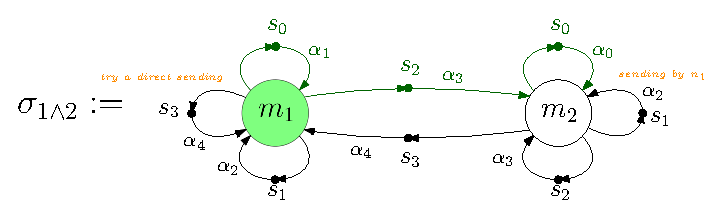
\includegraphics[width=0.7\linewidth]{resources/strategy2}
    \caption{Strategy representing a compromise between $\sigma_1$ and $\sigma_2$ for $\mathcal{M}$}
    \label{strat-compromise}
  \end{figure}
  Indeed, we assume that $\sigma_{1 \wedge 2}$ is initialised in the mode $m_1$ and first try a direct sending to $n_2$. If it fails, it then sends the message via $n_1$.
  As $\sigma_{1 \wedge 2}$ tries a direct sending to $n_2$,
    the cost of this try is $4$ $ms$, $394$ $mJ$ and succeeds with a probability $\frac{7}{8}$.
    If it fails, the strategy next sends the message via $n_1$ and the time threshold is exceeded.
    It does however not matter because the probability threshold to reach $s_3$ within $4$ $ms$ is satisfied. Then, assuming the direct sending has failed, the message is sent via $n_1$. In that case, the total cost of the sending is thus exactly $394 + 296 = 690 < 700$ $mJ$. Thus,
  \begin{itemize}
    \item $\mathbb{P}_{s_0}^{\sigma_{1 \wedge 2}}(\Diamond_{1:\, \leq 4}\, \{s_3\}) = 0.875 \geq 0.8 \implies \sigma_{1 \wedge 2} \text{ satisfies }\mathcal{Q}_1, \text{ and}$
    \item $\mathbb{P}_{s_0}^{\sigma_{1 \wedge 2}}(\Diamond_{2:\, \leq 700}\, \{s_3\}) = 1 \geq 0.9 \implies \sigma_{1 \wedge 2} \text{ satisfies }\mathcal{Q}_2.$
  \end{itemize}

Assume now that we want to additionally ensure that the message will be sent and acknowledged within $8$ $ms$ with a probability of $0.9$.
That yields the following \SSPPQ{} problem:
\[
  ?\exists \sigma \;\; \mathbb{P}^{\sigma}_{s_0}(\Diamond_{1: \, \leq 4} \, \{s_3\}) \geq 0.8 \; \wedge \;
   \mathbb{P}^{\sigma}_{s_0}(\Diamond_{1: \, \leq 8} \, \{s_3\}) \geq 0.9 \; \wedge \;
  \mathbb{P}_{s_0}^{\sigma}(\Diamond_{2: \, \leq 700} \, \{s_3\}) \geq 0.9
\]
None pure strategy can satisfy simultaneously these percentile queries, even finite-memory strategies.
In order to satisfy this \SSPPQ{} problem, we additionally need the notion of randomisation in our strategies.
\end{example}

Let $\mathcal{M}=(S, A, \Delta, w, AP, L)$ be a $d$-dimensional MDP,
$s^* \in S$, and $q \in \mathbb{N}$ percentile constraints described by
$T_i \subseteq S$, the dimension $k_i \in \{1, \dots, d\}$, the cost threshold $\ell_i \in \mathbb{N}$, and the probability threshold $\alpha_i \in [0, 1] \cap \mathbb{Q}$, for each constraints $i \in \{1, \dots, q\}$.
We will now introduce an algorithm to solve the \SSPPQ{} problem for the state $s^*$ and these $q$ constraints. This algorithm allows to build an optimal strategy with both finite-memory and randomisation to satisfy the problem.
Note that we assume all dimensions of $\mathcal{M}$ being relevant for this problem, i.e., $\bigcup_{i \in \{1, \dots q\}} k_i = \{1, \dots, d\}$.
On the other hand, we simply drop the $n$ irrelevant dimensions of $\mathcal{M}$ for the problem and we only consider the $d-n$ remaining one.
In order to describe this algorithm, we need to define the \textit{multi-dimensional unfolding of an MDP}.

\begin{definition}[\textbf{Multi-dimensional unfolding of an MDP}]
The \textit{$d$-dimensional unfolding of the MDP $\mathcal{M}$ from the state $s^*$
up to the highest cost threshold of $(\ell_i)_{i \in \{1, \dots, q\}}$ on each dimension of $(k_i)_{i \in \{1, \dots, q\}}$} is a $1$-dimensional MDP \sloppy $\mathcal{M}' = {(S', A', \Delta', AP, L')}$ defined as follows:
  \begin{itemize}
    \item $S' \subseteq S \times (\{ 0, \dots, \ell^{\max} \} \cup \{\bot\})^d$, with $\ell^{\max} = \max_{i \in \{1, \dots, q\}}\ell_i$,  is the set of states composed of states $(s, v_1, \dots, v_d)$ such that $s \in S$ and, for each dimension $k \in \{1, \dots, d\}$, $v_k \in \{0, \dots, \ell^{\max}_k\} \cup \{\bot\}$, where $\ell^{\max}_k$ is the maximum threshold on the dimension $k$, i.e., \[\ell^{\max}_k = \max_{i \in \{1, \dots, q\} \; | \; k_i = k }  \, \ell_i,\]
    and we consider that $\bot > \ell_k^{\max}$
    and $\bot + v = \bot$, for all $v \in \mathbb{N}$.
    Intuitively, the vector $(v_1, \dots, v_d)$ records the cost of paths on all the dimensions while unfolding $\mathcal{M}$.
    \item $A'$ is the set of action of the unfolding such that $\alpha \in A'$
    for all actions $\alpha \in A$, and
    $A'(s, v_1, \dots, v_d) = A(s)$
    for all $(s, v_1, \dots, v_d) \in S'$.
    \item $\Delta'$ is the probability transition function defined as follows: let $x = (s, v_1, \dots, v_d) , \, x'=(s', v'_1, \dots, v'_d) \in S'$, $\alpha \in A'(s)$,
    and
    $succ_k: S' \times A' \rightarrow \{0, \dots, \ell^{\max}_k\},$
    \[((s, v_1, \dots, v_d), \, \alpha) \mapsto \begin{cases}
      v_k + w_k(\alpha) & \text{if } v_k + w_k(\alpha) \leq \ell^{\max}_k \\
      \bot & \text{else},
    \end{cases}\]
    referring to the $\alpha$-successor of $(s, v_1, \dots, v_d)$ on the cost dimension $k \in \{1, \dots, d\}$,
    \[
    \Delta'(x, \alpha, x') = \begin{cases}
      \Delta(s, \alpha, s') & \text{if } \forall k \in \{1, \dots, d\}, \, v'_k = succ_k(x) \\
      & \quad \text{and }\exists k \in \{1, \dots, d\}, \, v_k \neq \bot, \\
      \sum_{s'' \in S} \Delta(s, \alpha, s'')
      & \text{if } \forall k \in \{1, \dots, d\},\, succ_k(x) = \bot \\
      & \quad \text{and } x \neq x', \, x' = s_\bot,\\
      1 & \text{if } x=x'=s_\bot \text{ and } \alpha = \alpha_\bot, \\
      0 & \text{otherwise,}
    \end{cases}
    \]
    where $s_\bot$ represents the state for which the cost thresholds have been exceeded on all the dimensions, i.e., where for all $k \in \{1, \dots, d\}$, $v_k = \bot$. We consider that this state has only one enabled action $\alpha_\bot$.
    \item $L': S' \rightarrow AP,\, (s, v_1, \dots, v_d) \mapsto L(s)$ is the labelling function of the unfolding.
  \end{itemize}
    Furthermore, as we unfold $\mathcal{M}$ from $s^*$, we limit the state space $S'$ with the states reachable from $(s^*, 0, \dots, 0)$.
\end{definition}

This definition allows us to describe an algorithm defined to solve the \SSPPQ{} problem for the state $s^*$ and the $q$ constraints (cf. Algorithm \ref{ssppq-algo}).

\begin{algorithm}
\caption{Solving the \SSPPQ{} problem}\label{ssppq-algo}
\begin{enumerate}
\item We build the MDP $\mathcal{M}'$, being the $d$-dimensional unfolding of $\mathcal{M}$ up to the highest cost thresholds on each of these dimensions.
  A path is thus discarded only if its current cost exceeds all highest threshold on each of these dimensions.
  Indeed, some paths exceeding the cost threshold of a request could still interesting to satisfy the others.
  \item Then, we compute the set of target states \[T'_i = \{ (s, v_1, \dots, v_d) \in S' \; | \; s \in T_i  \; \wedge \; v_{k_i} \leq l_i \}\] in $\mathcal{M}'$ for each request $i \in \{1, \dots, q\}$.
  \item Finally, we are left with a \MOSR{} problem on $\mathcal{M}'$: we are looking for a strategy ensuring that each of these sets $T'_i$ are reached from $(s^*, 0, \dots, 0)$ with a probability $\alpha_i$ (cf. Section \ref{mosr-section}).
\end{enumerate}
\end{algorithm}

\begin{remark}[\textit{\SSPPQ{} problem with single-target queries}] \label{remark-sspp}
  Assume that all constraints are described by the same set of target states, i.e., $\forall i \in \{1, \dots, r\}$, $\cup_{j=1}^r T_j = T_i$.
  In that case, as soon as a path visit a target state in the unfolding, it is not useful to consider and visit successors of this target state until that the highest cost thresholds have been exceeded on all the dimensions.
  Indeed, remind that given any prefix of a path, extending it can never decrease its current cost %regarding to the cost of this prefix
  (the weights are strictly positive).\par
  Thus, under the assumption that the constraints of an \SSPPQ{} problem for a given MDP have the same set of target states, we can make absorbing all of these states in the unfolding to avoid visiting some useless states.
  Solving this \SSPPQ{} problem is then polynomial in the multi-dimensional unfolding of the MDP (cf. Corollary \ref{mosr-absorbing-cor}).
\end{remark}

\begin{theorem}[\textit{\textbf{Solving the \SSPPQ{} problem}}]
  The \SSPPQ{} problem
  can be solved in general in polynomial time in the size of $\mathcal{M}$ and exponential time in the query size (exponential in the number of constraints and pseudo-polynomial in the length of the largest threshold). Furthermore, it
  can be decided in pseudo-polynomial time in the size of $\mathcal{M}$ and in the length of the highest threshold for simultaneously single-dimension and single-target queries (cf. Remark \ref{remark-sspp}, and Corollary \ref{mosr-absorbing-cor}).
  Randomised exponential-memory strategies are always sufficient and in general necessary.
  %A satisfying strategy can be built in exponential time.
\end{theorem}

\begin{example}[\textit{\SSPPQ{} problem in the wireless sensor network}]
  We apply Algorithm \ref{ssppq-algo} to answer to the percentile request left open in Example \ref{SSPQ-example1}:
  \[
  ?\exists \sigma \;\; \underbrace{\mathbb{P}^{\sigma}_{s_0}(\Diamond_{1: \, \leq 4} \, \{s_3\}) \geq 0.8}_{\mathcal{Q}_1} \; \wedge \;
   \underbrace{\mathbb{P}^{\sigma}_{s_0}(\Diamond_{1: \, \leq 8} \, \{s_3\}) \geq 0.9}_{\mathcal{Q}_2} \; \wedge \;
  \underbrace{\mathbb{P}_{s_0}^{\sigma}(\Diamond_{2: \, \leq 700} \, \{s_3\}) \geq 0.9}_{\mathcal{Q}_3}
  \]
  In order to solve this \SSPPQ{} problem, we build the $2$-dimensional unfolding $\mathcal{M'}$ of the MDP of Figure \ref{multi-mdp}, for the state $s_0$, the cost thresholds $\ell_1 = 4$, $\ell_2 = 8$, $\ell_3 = 700$, and the dimensions $k_1 = k_2 = 1$, $k_3 = 2$ (cf. Figure \ref{multi-unfolding}).
  \begin{figure}[h]
    \centering
    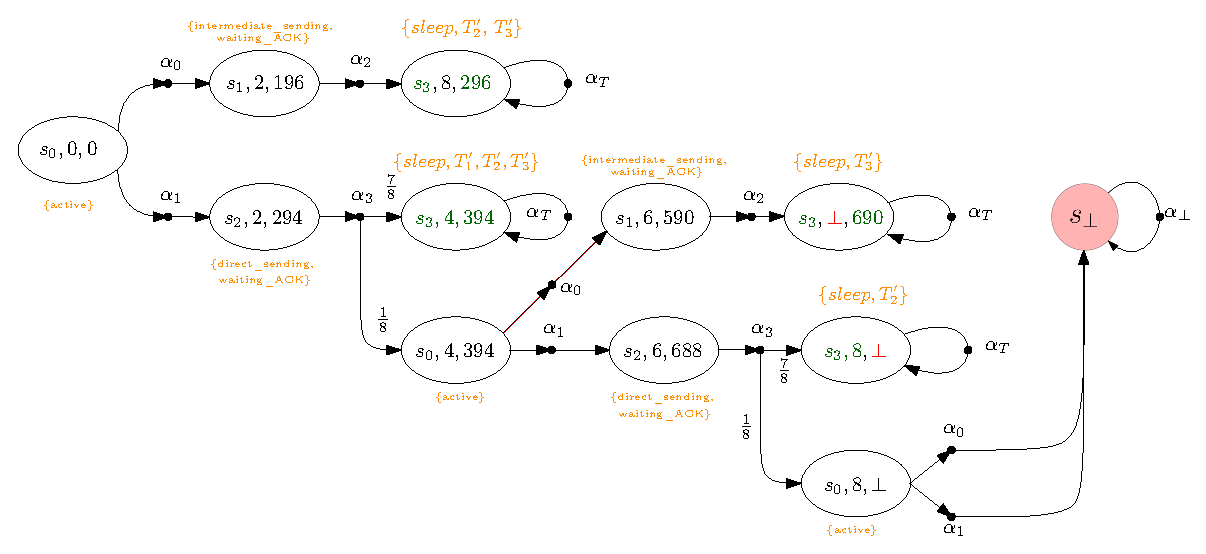
\includegraphics[width=\linewidth]{resources/SSP-PQ-unfolding}
    \captionsetup{justification=centering}
    \caption{Unfolding of the MDP of Figure \ref{multi-mdp} from $s_0$ up to the cost thresholds $4$ and $8$ on the time dimension, and $700$ on the energy dimension}
    \label{multi-unfolding}
  \end{figure}
  As each constraint describes a percentile problem,
  and as the set of target states for all constraints is $\{s_3\}$, we do not need to consider states after that $\{s_3\}$ is reached in all paths starting from $(s_0, 0, 0)$ in $\mathcal{M}'$.
  We can thus make all states referring to $s_3$  absorbing in $\mathcal{M}'$ (cf. Remark \ref{remark-sspp}).
  The new sets of target states are $T'_1 = \{(s_3, 4, 394)\}$, $T'_2 = \{(s_3, 8, 296), \, (s_3, 4, 394), \, (s_3, 8, \bot)\}, \, T'_3 = \{ (s_3, 8, 296), \, (s_3, 4, 494) \}$
  for all query $\mathcal{Q}_i$, with $i \in \{1, \dots, 3\}$. As all target states are absorbing, we can build a satisfying randomised memoryless optimal strategy in polynomial time in the size of $\mathcal{M}'$ (cf. Corollary \ref{mosr-absorbing-cor}).
  %The randomised memoryless strategy $\sigma$ such that $\sigma(s')(\alpha) = 1$ for all $s' \in S'$ such that $\alpha \in A(s)$, $|A(s)| = 1$, and
  %$\sigma((s, 0, 0))(\alpha_1) = 1$, $\sigma((s_0, 4, 394))(\alpha_0) = \sigma((s_0, 4, 394))(\alpha_1) = \frac{1}{2}$ satisfies the problem.
  We build the randomised memoryless strategy
  \[
  \sigma(s')(\alpha) = \begin{cases}
    1 & \text{if } \alpha \in A(s) \text{ and } |A(s)| = 1,
    \text{ or if } s'=(s_0, 0, 0) \text{ and } \alpha=\alpha_1, \\
    \frac{1}{2} & \text{if } s'=(s_0,4,394) \text{ and } \alpha \in \{\alpha_0, \alpha_1\},\\
    0 & \text{otherwise}.
  \end{cases}
  \]
  The MC induced by $\sigma$ is given on Figure \ref{mc-unfolding}.
  \begin{figure}[h]
    \centering
    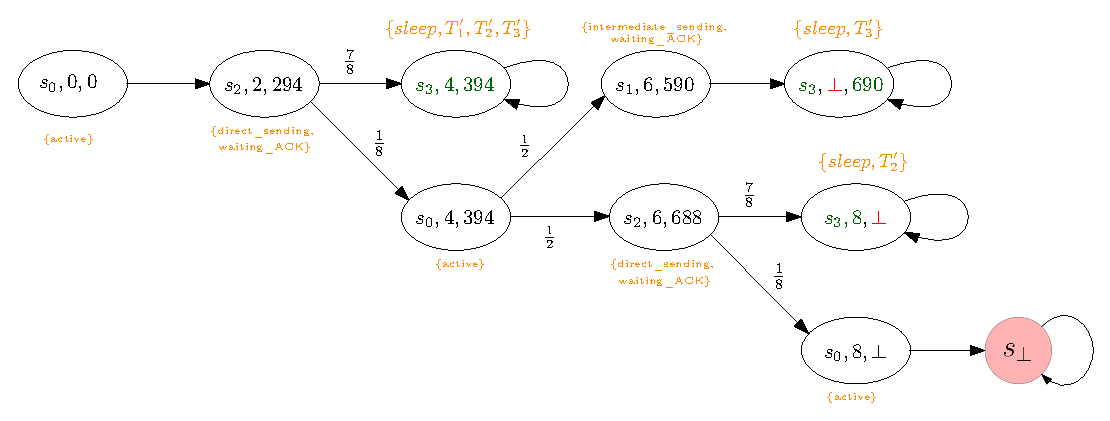
\includegraphics[width=\linewidth]{resources/SSP-PQ-unfolding2}
    \caption{Product of $\sigma$ with $\mathcal{M}'$, yielding the induced MC by $\sigma$}
    \label{mc-unfolding}
  \end{figure}
  We have $\mathbb{P}^\sigma_{(s_0, 0, 0)}(\Diamond T'_1) = \frac{7}{8}$, $\mathbb{P}^\sigma_{(s_0, 0, 0)}(\Diamond T'_2) = \frac{7}{8} + \frac{1}{8} \cdot \frac{1}{2} \cdot \frac{7}{8} \geq 0.9$, and
  $\mathbb{P}^\sigma_{(s_0, 0, 0)}(\Diamond T'_3) = \frac{7}{8} + \frac{1}{8} \cdot \frac{1}{2} \geq 0.9$. Thus, we have that $\sigma$ satisfies $\mathcal{Q}_1$, $\mathcal{Q}_2$, and $\mathcal{Q}_3$.
  The strategy $\sigma$ is memoryless in $\mathcal{M}'$, and exponential-memory in $\mathcal{M}$.
  Thus, the \SSPPQ{} problem is solved.
\end{example}
